% Dies ist ein Beispiel-Tex-File f\"{u}r eine wissenschaftliche Arbeit
% Es kann nach Belieben ver\"{a}ndert werden
% Die Präambel ist größtenteils ausgelagert
% Details zu den Paketen sind den entsprechenden Dokus zu entnehmen
% Insbesondere die KOMA-Skript-Doku sollte jeder mal angeschaut haben
% Erstellt von K. Holste f\"{u}r den PTRA-Studiengang

% Festlegung der Dokumentklasse
\documentclass[fontsize=11pt,%
twoside,% oneside als Alternative m\"{o}glich
BCOR          = 8mm, % bei Bedarf anzupassen
DIV           = 11,  % kann nach Belieben geändert werden
titlepage     = off,%
index=totoc,%
xcolor        = pdftex,%
dvipsnames,%
%bibliography  = totoc,%
%bibliography = numbered,% bei Bedarf einschalten
listof        = notnumbered]{scrreprt}



\newif\ifdesignEins
\newif\ifdesignZwei
\newif\ifdesignDrei
\newif\ifjournalabbrev % variablendeklaration.tex wird benötigt (für verschiedene Layouts der Kapitelseite)

% Layout der Kapitelseite kann hier geändert werden
% werden alle drei Optionen ausgeklammert (mit %), wird KOMA-Default verwendet:

%\designEinstrue
%\designZweitrue
\designDreitrue

% Hier geht es um abgekürzte Journal-Namen
% True = Journalnamen werden abgekürzt, sofern Abkürzungsfeld vorhanden (shortjournal)
% False = keine Abkürzung (es reicht, die folgende Zeile auszukommentieren)
\journalabbrevtrue

% Einbindung von wichigten Paketen
\usepackage[headsepline=on, automark]{scrlayer-scrpage}
\usepackage[english, main=ngerman]{babel}  % Assuming you're using both German and English
\usepackage[utf8]{inputenc}
\usepackage[T1]{fontenc}
\usepackage{lmodern}
%\usepackage{fourier} % Adobe Utopia Font
\usepackage{microtype}
%\microtypesetup{expansion=false} % bei Verwendung von fourier eventuell notwendig
\usepackage{scrdate}
\usepackage{scrtime}
\usepackage{lastpage}
\usepackage{upgreek}
\usepackage[svgnames]{xcolor}
\usepackage{blindtext} % Erzeugt Blindtext. Nur f\"{u}r Testlauf dieses Dokuments wichtig.
\usepackage{graphicx}
\usepackage{siunitx}
\usepackage{booktabs}
\usepackage{longtable}
\usepackage{threeparttable}
\usepackage{typearea}
\usepackage{tikz}
\usepackage{tikzpagenodes}
\usepackage{epigraph}
\usepackage{ellipsis}
\usepackage{soul}
\usepackage[nohyperlinks]{acronym}
\usepackage[autostyle,german=guillemets]{csquotes}
\usepackage[defaultlines = 4, all]{nowidow}
\clubpenalty = 9999
\widowpenalty = 9999
\displaywidowpenalty = 9999
\usepackage{eurosym}

% Die AMS-Mathe-Pakete
\usepackage{amsmath}
\usepackage{amsthm}
\usepackage{amsfonts}
%%%%%%%%%%%%%%%%%%%%%

\usepackage{setspace}
\usepackage{hyperref} % immer als letztes Paket laden
% Hintergrundvariablen des PDFs
\hypersetup{pdfauthor={Martina Musterfrau},
            pdftitle={Abschlussarbeit},
            pdfsubject={Abschlussarbeit},
            pdfkeywords={Abschlussarbeit PTRA},
            pdfproducer={Latex with hyperref},
            pdfcreator={pdflatex, MikTeX, WinEDT oder andere}
            }


% Marcel packages
\usepackage{float}  % Include the float package for [H] float positioning
% Redefine "Kapitel" to "Chapter"
\addto\captionsngerman{
  \renewcommand{\chaptername}{Chapter}
}
% Redefine the figure caption label from "Abbildung" to "Figure"
\addto\captionsngerman{
  \renewcommand{\figurename}{Figure}
}


% Farbdefinitionen
\definecolor{jluhellblau}{RGB}{220, 230, 235}
\definecolor{pantoneblack}{RGB}{0,0,0}
\definecolor{jlugrau}{RGB}{83, 96, 107}
\definecolor{jlublau}{RGB}{0, 105, 179}
\definecolor{chaptergrey}{rgb}{0.7,0.7,0.7}
\definecolor{thmgreen}{RGB}{128,186,36}
\definecolor{thmgrau}{RGB}{74,92,102}
\definecolor{thmblau}{RGB}{0,59,209}
\definecolor{thmbhellblau}{RGB}{64,255,237}



% Kopf- und Fu{\ss}zeilenlayout
\clearpairofpagestyles
\automark[chapter]{chapter}
\automark*[section]{}
\ihead{}
\ohead{\headmark}
\ifoot{Erstellt am \ISOToday T\thistime} % f\"{u}r finales Dokument auskommentieren
%\ifoot{} % f\"{u}r finales Dokument aktivieren
\ofoot{\,\pagemark\ von \pageref*{LastPage}}
\chead{}
\cfoot[]{}

% Fu{\ss}notenmarker fett
\deffootnote{1em}{1em}{\bfseries\thefootnotemark\ }

% Formatierung Tabellen- und Abbildungsbeschriftung
\setcapindent{0pt} % keine Einr\"{u}ckung der Caption
\renewcommand{\floatpagefraction}{1.0}
\addtokomafont{caption}{\footnotesize}
\setkomafont{captionlabel}{\bfseries\sffamily}

% Literaturverzeichnis mit BibLaTeX
\usepackage[backend = biber, style=numeric-comp, sorting = none, giveninits = true]{biblatex}
\ifjournalabbrev
\usepackage{biblatex-shortfields}
\else\fi

\DefineBibliographyStrings{ngerman}{andothers = {{et\,al\adddot}},}
\addbibresource{references.bib}




% Es ist im Literaturverzeichnis unn\"{o}tig, DOI, URL und eprint gleichzeitig zu zeigen. Dieser Abschnitt macht eine
% Fallunterscheidung. Ist die DOI vorhanden, werden URL und eprint nicht angezeigt. Ist DOI nicht vorhanden, aber
% die beiden anderen Eintr\"{a}ge, wird die URL ausgegeben, nicht aber der eprint-Eintrag.
\renewbibmacro*{doi+eprint+url}{%
  \iftoggle{bbx:doi}
    {\printfield{doi}}
    {}%
  \newunit\newblock
  \ifboolexpr{togl {bbx:eprint} and test {\iffieldundef{doi}}}
    {\usebibmacro{eprint}}
    {}%
  \newunit\newblock
  \ifboolexpr{togl {bbx:url} and test {\iffieldundef{doi}}  and test {\iffieldundef{eprint}}}
    {\usebibmacro{url+urldate}}
    {}}
\renewbibmacro{in:}{%
  \ifentrytype{article}{}{\printtext{\bibstring{in}\intitlepunct}}}
% Ende Literaturverzeichnis-Definitionen

% Start Kapitelseiten-Designs
\ifdesignEins
\addtokomafont{chapterprefix}{\raggedleft}
\renewcommand*{\chapterformat}{%
\mbox{\chapappifchapterprefix{\nobreakspace}%
\scalebox{3}{\color{chaptergrey}\thechapter\autodot}\enskip}}
\else
\fi
\newif\ifdesignEins
% zweites Design
\ifdesignZwei
\setkomafont{chapter}{\huge}
\setkomafont{chapterprefix}{\normalfont\normalsize\slshape}
\newkomafont{chapternumber}{\fontsize{100}{100}\selectfont}
\renewcommand\chapterformat{%
  \usekomafont{chapter}
  \raisebox{1.25\baselineskip}{\makebox[0pt][r]{\usekomafont{chapterprefix}\chapapp\enskip}}%
  \raisebox{-.5\baselineskip}{\usekomafont{chapternumber}\thechapter}%
}
\RedeclareSectionCommand[
  innerskip=1ex
]{chapter}
\newbox\chapternumberbox
\makeatletter
\renewcommand\chapterlinesformat[3]{%
  \Ifstr{#1}{chapter}{%
    \Ifstr{#2}{}{#3}{%
      \savebox\chapternumberbox{\chapterformat}%
      \parbox[t]{\dimexpr\textwidth-\wd\chapternumberbox-1em\relax}{\raggedchapter#3}%
       \quad#2%
    }%
    }{\@hangfrom{#2}{#3}}%
}
\makeatother
\renewcommand\raggedchapter{\raggedleft}
\else
\fi
\ifdesignDrei
\makeatletter
 \renewcommand*{\chapterformat}{%
   \begingroup
     \setlength{\unitlength}{1mm}%
     \begin{picture}(10,10)(0,5)
       \setlength{\fboxsep}{0pt}
       \put(10,15){\line(1,0){\dimexpr
           \textwidth-20\unitlength\relax\@gobble}}%
       \put(0,0){\makebox(10,20)[r]{%
           \fontsize{28\unitlength}{28\unitlength}\selectfont\thechapter
           \kern-.05em% Ziffer in der Zeichenzelle nach rechts schieben
         }}%
       \put(10,15){\makebox(\dimexpr
           \textwidth-20\unitlength\relax\@gobble,\ht\strutbox\@gobble)[l]{%
             \ \normalsize\color{black}\chapapp~\thechapter\autodot
           }}%
     \end{picture}
   \endgroup
}
\else
\fi
% Ende des Kapitelseiten-Designs

% L\"{o}st ein Problem, dass Abbildungen ans Ende des Kapitels schiebt
\renewcommand{\floatpagefraction}{0.8}
\renewcommand{\topfraction} {0.8}
\renewcommand{\bottomfraction} {0.5}
\renewcommand{\textfraction} {0.15}
\raggedbottom

% Neuberechnung des Satzspiegels nach Defintion aller Parameter
\recalctypearea

% Soll Schusterjungen verhindern
\noclub

\pdfminorversion=7

% Wenn man die Kurzform der Journalnamen verwenden will, sind folgende Zeilen nützlich.
% z.B. einfach \actaa in shortjorunal einsetzen, erzeugt Acta.Astron.

\newcommand{\actaa}{Acta Astron.}   % Acta Astronomica
\newcommand{\araa}{Annu. Rev. Astron. Astrophys.}   % Annual Review of Astron and Astrophys
\newcommand{\aar}{Astron. Astrophys. Rev.} % Astrononmy and Astrophysics Review
\newcommand{\ab}{Astrobiol.}    % Astrobiology
\newcommand{\aj}{Astron. J.}   % Astronomical Journal
\newcommand{\apj}{Astrophys. J.}   % Astrophysical Journal
\newcommand{\apjl}{Astrophys. J. Lett.}   % Astrophysical Journal, Letters
\newcommand{\apjs}{Astrophys. J. Suppl. Ser.}   % Astrophysical Journal, Supplement
\newcommand{\ao}{Appl. Opt.}   % Applied Optics
\newcommand{\apss}{Astrophys. Space Sci.}   % Astrophysics and Space Science
\newcommand{\aap}{Astron. Astrophys.}   % Astronomy and Astrophysics
\newcommand{\aapr}{Astron. Astrophys. Rev.}   % Astronomy and Astrophysics Reviews
\newcommand{\aaps}{Astron. Astrophys. Suppl.}   % Astronomy and Astrophysics, Supplement
\newcommand{\baas}{Bull. Am. Astron. Soc.}   % Bulletin of the AAS
\newcommand{\caa}{Chinese Astron. Astrophys.}   % Chinese Astronomy and Astrophysics
\newcommand{\cjaa}{Chinese J. Astron. Astrophys.}   % Chinese Journal of Astronomy and Astrophysics
\newcommand{\cqg}{Class. Quantum Gravity}    % Classical and Quantum Gravity
\newcommand{\gal}{Galaxies}    % Galaxies
\newcommand{\gca}{Geochim. Cosmochim. Acta}   % Geochimica Cosmochimica Acta
\newcommand{\icarus}{Icarus}   % Icarus
\newcommand{\jcap}{J. Cosmol. Astropart. Phys.}   % Journal of Cosmology and Astroparticle Physics
\newcommand{\jgr}{J. Geophys. Res.}   % Journal of Geophysics Research
\newcommand{\jgrp}{J. Geophys. Res.: Planets}    % Journal of Geophysics Research: Planets
\newcommand{\jqsrt}{J. Quant. Spectrosc. Radiat. Transf.} % Journal of Quantitiative Spectroscopy and Radiative Transfer
\newcommand{\memsai}{Mem. Soc. Astron. Italiana}   % Mem. Societa Astronomica Italiana
\newcommand{\mnras}{Mon. Not. R. Astron. Soc.}   % Monthly Notices of the RAS
\newcommand{\nat}{Nature} % Nature
\newcommand{\nastro}{Nat. Astron.} % Nature Astronomy
\newcommand{\ncomms}{Nat. Commun.} % Nature Communications
\newcommand{\nphys}{Nat. Phys.} % Nature Physics
\newcommand{\na}{New Astron.}   % New Astronomy
\newcommand{\nar}{New Astron. Rev.}   % New Astronomy Review
\newcommand{\physrep}{Phys. Rep.}   % Physics Reports
\newcommand{\pra}{Phys. Rev. A}   % Physical Review A: General Physics
\newcommand{\prb}{Phys. Rev. B}   % Physical Review B: Solid State
\newcommand{\prc}{Phys. Rev. C}   % Physical Review C
\newcommand{\prd}{Phys. Rev. D}   % Physical Review D
\newcommand{\pre}{Phys. Rev. E}   % Physical Review E
\newcommand{\prl}{Phys. Rev. Lett.}   % Physical Review Letters
\newcommand{\psj}{Planet. Sci. J.}   % Planetary Science Journal
\newcommand{\planss}{Planet. Space Sci.}   % Planetary Space Science
\newcommand{\pnas}{Proc. Natl Acad. Sci. USA}   % Proceedings of the US National Academy of Sciences
\newcommand{\procspie}{Proc. SPIE}   % Proceedings of the SPIE
\newcommand{\pasa}{Publ. Astron. Soc. Aust.}   % Publications of the Astron. Soc. of Australia
\newcommand{\pasj}{Publ. Astron. Soc. Jpn}   % Publications of the Astron. Soc. of Japan (note no full stop following Jpn)
\newcommand{\pasp}{Publ. Astron. Soc. Pac.}   % Publications of the Astron. Soc. of the Pacific
\newcommand{\rsi}{Rev. Sci. Instrum.}   % Review of Scientific Instruments
\newcommand{\rmxaa}{Rev. Mexicana Astron. Astrofis.}   % Revista Mexicana de Astronomia y Astrofisica
\newcommand{\sci}{Science} % Science
\newcommand{\sciadv}{Sci. Adv.} % Science Advances
\newcommand{\solphys}{Sol. Phys.}   % Solar Physics
\newcommand{\sovast}{Soviet Ast.}   % Soviet Astronomy
\newcommand{\ssr}{Space Sci. Rev.}   % Space Science Reviews
\newcommand{\uni}{Universe} % Universe  % preambel.tex wird benötigt

\pagestyle{empty}

\begin{document}
\newcommand{\boldvec}[1]{\bm{#1}}


% Schmutztitel im einseitigen Layout
% Schmutztitel wird einseitig gesetzt, um Layout
% nicht zu zerschreddern
% Wer den Schmutztitel nicht haben will, l\"{o}scht diesen Teil einfach
\KOMAoptions{twoside=false}
% Beginn des Schmutztitels als Teil der Titlepage-Umgebung
\begin{titlepage}%Schmutztitel; Grafiken mit Tikz erstellt; Signet eingebunden
\begin{tikzpicture}[remember picture,overlay,shift={(current page.south)}]


\fill[left color=thmgreen, right color=jluhellblau] (-9,10) rectangle +(20,15.5);

\node at (7.5,25.5) {
\includegraphics[width = 0.32\textwidth]{logo1.jpg}};
\node at (-2.5,26.8) {
\includegraphics[width = 0.85\textwidth]{THM_logo.eps}};

\fill[left color=jlublau!100, right color=jlublau!100](-10,5) rectangle +(17.5,6);

\node [text width=14cm] at (-1.0, 8.4)
{
\sffamily
\color{white}
\begin{center}
\Large
\textbf{Bachelorarbeit}\\[1.1ex]
\LARGE
\textbf{Experimentelle Untersuchungen zum Beamen während des Fliegens mit Warp-Geschwindigkeit}\\[1.1ex]
\Large
\textbf{Experimental studies on beaming while flying at warp speed}\\[1.1ex]
\textbf{Martina Musterfrau}\\[1.2ex]
\Large
\textbf{Sommersemester 2021}
\end{center}
};

\node [text width=4cm] at (9.75,2){\LARGE \sffamily \color{black}{\textbf{P}}\color{thmgreen}{\textbf{T}}\color{jlublau}{\textbf{R}}\color{black}{\textbf{A}}};

% Auskommentieren erzeugt Hilfslinien und Punkte auf Schmutztitelseite
% kann hilfreich für Anpassungen sein
%\draw [help lines] (-10,0) grid (10,30);
%\draw [fill=black] (0, 0) circle (0.1);
%\draw [fill=black] (0, 5) circle (0.1);
%\draw [fill=black] (0, 10) circle (0.1);
%\draw [fill=black] (0, 15) circle (0.1);
%\draw [fill=black] (0, 20) circle (0.1);
%\draw [fill=black] (0, 25) circle (0.1);
%\draw [fill=black] (5, 0) circle (0.1);
%\draw [fill=black] (5, 5) circle (0.1);
%\draw [fill=black] (5, 10) circle (0.1);
%\draw [fill=black] (5, 15) circle (0.1);
%\draw [fill=black] (5, 20) circle (0.1);
%\draw [fill=black] (5, 25) circle (0.1);
%\draw [fill=black] (-10, 0) circle (0.1);
%\draw [fill=black] (-10, 5) circle (0.1);
%\draw [fill=black] (-10, 10) circle (0.1);
%\draw [fill=black] (-10, 15) circle (0.1);
%\draw [fill=black] (-10, 20) circle (0.1);
%\draw [fill=black] (-10, 25) circle (0.1);
%\draw [fill=black] (-5, 0) circle (0.1);
%\draw [fill=black] (-5, 5) circle (0.1);
%\draw [fill=black] (-5, 10) circle (0.1);
%\draw [fill=black] (-5, 15) circle (0.1);
%\draw [fill=black] (-5, 20) circle (0.1);
%\draw [fill=black] (-5, 25) circle (0.1);
%\draw [fill=black] (10, 0) circle (0.1);
%\draw [fill=black] (10, 5) circle (0.1);
%\draw [fill=black] (10, 10) circle (0.1);
%\draw [fill=black] (10, 15) circle (0.1);
%\draw [fill=black] (10, 20) circle (0.1);
%\draw [fill=black] (10, 25) circle (0.1);




\end{tikzpicture}
\end{titlepage}
% Ende des Schmutztitels  % schmutztitel.tex wird benötigt

% ab hier wieder zweiseitiges Format
\KOMAoptions{twoside=true}

% richtige Titelseite; Ausrichtung an Satzspiegel
%% Titlepage
%  Note: all text inside < ... > has to be adapted!
{% enclose this page so what is defined here does not spill over elsewhere
\pagestyle{empty}
\setstretch{1.5}
\sffamily
%\hfill\includegraphics{logo_univie_bw}

\centering% the switch form will also prevent hyphenation which would be undesired for a title

\vfill
{\bfseries\Huge BACHELORARBEIT}

\vfill
Titel der Bachelorarbeit

{\LARGE\bfseries Experimentelle Untersuchungen zum Beamen während des Fliegens mit Warp-Geschwindigkeit}
\vfill

{\Large\bfseries Experimental studies on beaming while flying at warp speed}
\vfill

vorgelegt von

{\Large Martina Musterfrau}

\vspace{15mm}

zur Erlangung des akademischen Grades

{\Large Bachelor of Science (B.\,Sc.)}
\vfill


\vspace{15mm}

\raggedright
%\small
\centering
\begin{tabular}{p{0.25\textwidth}p{0.75\textwidth}}
Datum:          & \today \\[1.0ex]
Studiengang:    &  PTRA - Physik und Technologie f\"{u}r Raumfahrtanwendungen\\[1.0ex]
Matrikelnummer: &  123456789\\[1.0ex]
Erstgutachter:  &  Prof. Dr. Daniel D\"{u}sentrieb \\[1.0ex]
Zweitgutachter: &  Prof. Dr. Liten Hj\"{a}lpare \\
\end{tabular}
\cleardoublepage
% \end{titlepage}
}%end of title page  % titlepage.tex wird benötigt
\cleardoublepage

% Kopf- und Fußzeile wird aktiviert
\pagestyle{scrheadings}

% Korrektur Seitenzahl
% Muss eventuell korrigiert werden, so dass das
% Inhaltsverzeichnis die richtige Seitenzahl hat
%!!!!!!!!!!!!!!!!!!!!!!!!!!!!!!!!!!!!!!!!!!!!!!!
%\setcounter{page}{5} %!!!!!!!!!!!!!!!!!!!!!!!!!!
%!!!!!!!!!!!!!!!!!!!!!!!!!!!!!!!!!!!!!!!!!!!!!!!

% Inhaltsverzeichnis sowie weitere Verzeichnisse
\tableofcontents
\cleardoublepage

\pagenumbering{roman}
\listoffigures
\cleardoublepage

\listoftables
\cleardoublepage

\thispagestyle{plain}
\chapter*{Abbreviations}
\begin{acronym}
\acro{PIC}{\dotfill Particle-in-Cell}
\acro{ES PIC}{\dotfill Electrostatic Particle-In-Cell}
\acro{MCC}{\dotfill Monte Carlo Collisions}
\acro{DSMC}{\dotfill Direct Simulation Monte Carlo}
\acro{PDE}{\dotfill Partial Differential Equations}
\acro{FDM}{\dotfill Finite Difference Methods}
\acro{FEM}{\dotfill Finite Element Methods}
\acro{HOT}{\dotfill Higher-Order Terms}
\acro{GS}{\dotfill Gauss-Seidel}
\acro{SOR}{\dotfill Seccesive Over Relaxation}
%\acro{eugh}[ESA]{\dotfill European Space Agency}
%\acro{eu}[JLU]{\dotfill Justus-Liebig-Universit\"{a}t Gie{\ss}en}
\end{acronym}
\cleardoublepage

\selectlanguage{english}
\chapter*{Abstract}
\addcontentsline{toc}{chapter}{Abstract}
\markboth{Abstract}{}
\blindtext
\cleardoublepage

\selectlanguage{ngerman}
\chapter*{Zusammenfassung}
\addcontentsline{toc}{chapter}{Zusammenfassung}
\blindtext
\cleardoublepage % ben\"{o}tigt Abstract.tex

%%%%%%%%%%%%%%%%%%%%%%%%%%%%%%%%%%%%%%%%%%%%%%%%%%%%%%%%%%%%%%%
% Hier geht das Dokument richtig los
%%%%%%%%%%%%%%%%%%%%%%%%%%%%%%%%%%%%%%%%%%%%%%%%%%%%%%%%%%%%%%%


\chapter{Introduction}

Include here a short definition what plasma is and that we only used charged particles 

For the course of this research (other wording because already used) plasma is simply a gas containing charged particles in the form of ions and electrons




\section{Motivation}

\section{Research Objectives}


\section{Approach}
\chapter{Theoretical Framework}
In particle simulations, the behavior of charged particles is governed by the fundamental equations of motion derived from Newton's second law \cite{griffiths_introduction_2017}. The position and velocity of a particle change according to the following first-order differential equations \cite{brieda_plasma_2019}:
\begin{align}
    \frac{d\boldvec{r}}{dt} &= \boldvec{v}\\
    \frac{d\boldvec{v}}{dt} &= \frac{1}{m} \boldvec{F}
\end{align}

The first equation describes how the particle's position changes over time, equal to its velocity $\boldvec{v}$. The latter expresses the particle's acceleration $\boldvec{a}$, directly proportional to the net force $\boldvec{F}$ acting on it and inversely proportional to the particle's mass $m$.
\\

In the context of charged particles, a force arises from the interaction with the electric field $\boldvec{E}$ and magnetic field $\boldvec{B}$. This interaction is governed by the Lorentz force, which combines the effects of both fields to dictate the motion of a particle with a specific charge $q$:
\begin{align}
\boldvec{F}_{Lorentz} &= \boldvec{F}_{\text{electric}} + \boldvec{F}_{\text{magnetic}} \\
            &= q\boldvec{E} + q (\boldvec{v} \times \boldvec{B})
\end{align}

These fields are governed by the four fundamental equations of electromagnetism, known as Maxwell's equations. Generally, this set of partial differential equations relates the electric and magnetic fields to sources of charge and current, and is commonly expressed as \cite{zangwill_modern_2013}:
\begin{align}
\text{Gauss' law:} \quad & \nabla \cdot \boldvec{E} = \frac{\rho}{\epsilon_0} \\
\text{Gauss' law for magnetism:} \quad & \nabla \cdot \boldvec{B} = 0 \\
\text{Faraday's law:} \quad & \nabla \times \boldvec{E} = - \frac{\partial \boldvec{B}}{\partial t} \\
\text{Ampere's law:}\label{amperes law} \quad & \nabla \times \boldvec{B} = \mu_0 \left( \boldvec{j} + \epsilon_0 \frac{\partial \boldvec{E}}{\partial t} \right)
\end{align}

In this context, $\rho(\boldvec{r})$ represents the electric charge density, and $\boldsymbol{j}(\boldvec{r})$ refers to the current density. The constants $\varepsilon_0$ and $\mu_0$ are the vacuum permittivity and permeability, respectively.

For the scope of this research, we restrict the problem to an electrostatic assumption, where the magnetic field is assumed to be time-invariant. This assumption implies that the current density in the system is sufficiently low, such that corresponding to Amperes Law (see Eq. \ref{amperes law}) any self-induced magnetic field can be ignored. Additionally, the influence of gravity is negligible in this context, as it is multiple orders of magnitude weaker than the electrostatic forces acting on the particles. As a result, the force acting on the particles is reduced to the purely electrostatic force \cite{brieda_plasma_2019}, given by:
\begin{align}
\label{Electrostatic Force}\boldvec{F} &= q \boldvec{E}\\
\intertext{In electrostatics, the electric field \(\boldvec{E}\) is by convention the negative gradient of a scalar potential $\phi$: \cite{griffiths_introduction_2017}}
\label{E to Phi}\boldvec{E} &= - \nabla \phi\\
\intertext{Substituting that into Gauss’ law results in:}
\nabla \cdot (- \nabla \phi) &= \frac{\rho}{\epsilon_0}\\
\intertext{Finally, rearranging leads to the Poisson equation:}
\label{Eq: Poissions}\nabla^2 \phi &= - \frac{\rho}{\epsilon_0}
\end{align}
This powerful second-order partial differential equation relates the electric potential \(\phi\) to the charge distribution \(\rho\) in an electrostatic system. The objective of the subsequent sections is to find a solution for the electric potential under certain boundary conditions, thereby enabling the determination of the electric field (see Eq. \ref{E to Phi}). Subsequently, the electric field values can be used to update the position and velocity of all particles in the system through the corresponding electrostatic force (see Eq. \ref{Electrostatic Force}). This procedure is repeated until a predefined exit criterion is met, such as completing a specified simulation time or reaching a steady state (illustrated in Fig. \ref{fig: Flowchart}).
\\\newline
Alternatively, by applying Gauss’s Law to a single spherical charge distribution in electrostatics, the following expression for the electric field can be derived \cite{zangwill_modern_2013}:
\begin{equation}
\boldvec{E}_i = \frac{1}{4 \pi \epsilon_0} \sum_j^N q_j \frac{\boldvec{r}_i - \boldvec{r}_j}{\left| \boldsymbol{r}_i - \boldsymbol{r}_j \right|^3} \quad i \neq j
\end{equation}
This expression illustrates the superposition principle for discrete point charges, where the total electric field $\boldvec{E}_i$ at a given point $\boldvec{r}_i$ is the sum of the fields produced by each charge $q_j$. This also holds for a continuous charge distribution, where the sum is replaced by an integral over the region containing the charge. By utilizing the equation for the electrostatic force (see Eq. \ref{Electrostatic Force}), it is possible to derive the Coulomb force for a particle interacting with a total of $N$ charged particles:
\begin{align}
\boldvec{F}_{i} &= \frac{q_i }{4 \pi \epsilon_0} \sum_j^N q_j \frac{\boldvec{r}_i - \boldvec{r}_j}{|\boldvec{r}_i - \boldvec{r}_j|^3} \quad i \neq j
\end{align}

Conceptually, it would be possible to run a particle simulation by evaluating the Coulomb force for a system containing $N$ particles at each iteration step.  However, this direct approach is practically impossible due to the excessive computational and memory requirements, as it involves $N(N-1) \approx N^2$ force calculations per time step \cite{brieda_plasma_2019}. To overcome these challenges, the Particle-in-Cell (\acs{PIC}) method offers an efficient solution by computing the electric field throughout the system, thus significantly reducing computational complexity.

\begin{comment}    
One such approach is the use of macroparticles, which represent a stack of $w_m$ real ions or electrons moving in unison (discussed comprehensively in Section \textbf{!} \ref{sec: ES PIC}). The used simulation process is illustrated below:
\end{comment}

\usetikzlibrary{decorations.pathreplacing}
% Define a macro to collapse the grid drawing block
\newcommand{\drawGrid}{
    % Define the overlap length
    \def\overlap{0.3}
    
    % Draw full opacity dashed grid inside the 2x2 box
    \draw[black, dashed, opacity=1] (0,0) grid (2,2);
    
    % Draw reduced opacity dashed lines extending beyond the 2x2 box with adaptable length
    % Corner extensions
    \draw[black, dashed, opacity=0.3] (2,2) -- (2+\overlap,2);   % Right horizontal extension (top)
    \draw[black, dashed, opacity=0.3] (2,2) -- (2,2+\overlap);   % Top vertical extension (right)
    \draw[black, dashed, opacity=0.3] (0,2) -- (0-\overlap,2);   % Left horizontal extension (top)
    \draw[black, dashed, opacity=0.3] (0,2) -- (0,2+\overlap);   % Top vertical extension (left)
    \draw[black, dashed, opacity=0.3] (2,0) -- (2+\overlap,0);   % Right horizontal extension (bottom)
    \draw[black, dashed, opacity=0.3] (2,0) -- (2,0-\overlap);   % Bottom vertical extension (right)
    \draw[black, dashed, opacity=0.3] (0,0) -- (0-\overlap,0);   % Left horizontal extension (bottom)
    \draw[black, dashed, opacity=0.3] (0,0) -- (0,0-\overlap);   % Bottom vertical extension (left)
    
    % Middle line extensions
    \draw[black, dashed, opacity=0.3] (1,2) -- (1,2+\overlap);   % Middle top vertical extension
    \draw[black, dashed, opacity=0.3] (1,0) -- (1,0-\overlap);   % Middle bottom vertical extension
    \draw[black, dashed, opacity=0.3] (2,1) -- (2+\overlap,1);   % Middle right horizontal extension
    \draw[black, dashed, opacity=0.3] (0,1) -- (0-\overlap,1);   % Middle left horizontal extension
}

\section{Electrostatic Particle in Cell Method}
\label{sec: ES PIC}
As discussed in the previous section, the behavior of plasma in electrostatic fields is governed by Poisson’s equation (see Eq. \ref{Eq: Poissions}). This differential equation rarely has an analytical solution except in simple, idealized cases, requiring numerical methods for accurate simulation in complex practical applications. A common numerical method in this context is the Electrostatic Particle-In-Cell (\acs{ES PIC}) technique, which provides a valuable framework for plasma simulations and can even be extended to electromagnetic codes that solve Maxwell’s equations in their entirety \cite{brieda_plasma_2019}.

Unlike physical plasma phenomena, simulations proceed discontinuously by dividing the physical domain into a fine enough spatial grid. The individual elements of this computational grid are referred to as cells, which collectively form the simulation mesh. The points where the corners of these cells meet are known as nodes and are shared among neighboring cells. Generally, cells can have arbitrary shapes, provided they do not intersect with one another \cite{brieda_plasma_2019}. For the extent of this research, we used a quadratic cell layout in cartesian coordinates, which is advantageous due to its simplicity of implementation but lack the ability to resolve complex geometries. However, curved objects or smooth geometries can be implemented by using the sugarcube method, which allows for an approximation of complex shapes within a cartesian mesh (discussed in Section \ref{Chap: experimenantal part}).

Furthermore, the side length of a cell $\Delta x$ cannot be chosen excessively large but must instead be determined based on the specific objective and external conditions of the system. Generally, all plasmas can be characterized by a fundamental length, known as the Debye length $\lambda_\mathrm{d}$, which is determined by the temperature $T$ and number density $n$ of the charged particles \cite{gurnett_introduction_2017}. Considering a homogeneous plasma, where the ion temperature $T_\mathrm{i}$ is typically much lower than the electron temperature $T_\mathrm{e}$, it is customary to neglect the ion contribution \cite{brieda_plasma_2019}. This leads to the following expression for the Debye length: 
\begin{align}
\lambda_D = \sqrt{\frac{\epsilon_0 k_B T_e}{n_e q_e^2}}\quad\quad k_B &\text{: Boltzmann constant}\\
\intertext{To resolve the local charge density accurately and compute the electric field $\boldvec{E}$, the simulation grid must be sufficiently fine \cite{birdsall_plasma_2005}. Therefore, the cell volume in a \acs{PIC} simulation for plasma flow must be smaller than the volume of the Debye sphere, ensuring accurate resolution \cite{brieda_plasma_2019}:}
(\Delta x \Delta y \Delta z) &< \frac{4}{3} \pi \lambda_D^3
\end{align}

The simulation mesh intrinsically defines discrete points where key properties, such as the density $\rho$, the electric potential $\phi$, or the electric field $\boldvec{E}$, can be determined. While some methods define these points at the cell center, the commonly used node-based approach was employed in this work \cite{brieda_plasma_2019}. A particle within a cell interacts only with its surrounding nodes and is governed by the interpolated mesh data at its specific position within the cell. This approach accordingly enables the interpolation of particle-based data back onto the computational grid. Furthermore, the unique set of boundary conditions for the system is also established through the simulation mesh. Two of the most commonly applied boundary conditions in the context of \acs{PIC} simulations are the Dirichlet and Neumann boundary conditions. The Dirichlet boundary condition specifies the value of the function itself, such as the electric potential \cite{press_numerical_2007}. On the other hand, a Neumann boundary condition defines the values of the normal gradients on the boundary, implying that there is a predefined behavior in the direction perpendicular to the boundary \cite{press_numerical_2007}. Other types of boundary conditions include Robin, Cauchy, and mixed versions of both, though they are used less frequently in most applications \cite{brieda_plasma_2019}.

\begin{figure}[H]
    \centering
    \begin{tikzpicture}[scale=1.8]
    
    % Left Grid
    \drawGrid

    % Right Grid (shifted to the right by 4 units)
    \begin{scope}[xshift=4cm]
        \drawGrid
        \def\tolerance{0}

% Define the particle position
\def\particleX{1.6}
\def\particleY{0.8}

% Draw arrows from surrounding blue nodes to the green particle using 'latex' arrow tips
\draw[ thick, line width=1] (1+\tolerance,0+\tolerance) -- (\particleX-\tolerance,\particleY-\tolerance);  % Bottom-left node to particle
\draw[ thick, line width=1.1] (2-\tolerance,0+\tolerance) -- (\particleX+\tolerance,\particleY-\tolerance);  % Bottom-right node to particle
\draw[ thick, line width=1.5] (1+\tolerance,1-\tolerance) -- (\particleX-\tolerance,\particleY+\tolerance);  % Top-left node to particle
\draw[thick, line width=1.2] (2-\tolerance,1-\tolerance) -- (\particleX+\tolerance,\particleY+\tolerance);  
% Draw the particle
\fill[thmgreen,draw=black] (1.6,0.8) circle (3pt);  % Red particle with radius 3pt
\node[above] at (1, 2.3) {\textcolor{black}{cells}}; % Label "nodes" above the points

% Draw arrows from the "nodes" label to the blue points with a bit of spacing
\draw[-latex, thick] (.9, 2.3) -- (0.4, 1.5);  % Arrow to the leftmost blue point with some space
\draw[-latex, thick] (1.1, 2.3) -- (1.6, 1.5);  % Arrow to the middle blue point with some space

    \end{scope}

    % Draw the arrow and the text between the grids
    \draw[-latex,thick] (2.3,1) -- (3.7,1); % Arrow between the grid
    \node at (3,1.2) {next iteration};  % Text above the arrow

\draw[-latex,thick,red, line width=1.7] (0.45,0.3) -- (1.6,0.8) node[below] {$F_i$};

    % Define a tolerance for arrow starting and ending positions
\def\tolerance{0.00}

% Define the particle position
\def\particleX{0.4}
\def\particleY{0.3}

% Draw arrows from surrounding blue nodes to the green particle using 'latex' arrow tips
\draw[ thick, line width=0.8] (0+\tolerance,0+\tolerance) -- (\particleX-\tolerance,\particleY-\tolerance);  % Bottom-left node to particle
\draw[ thick, line width=1.1] (1-\tolerance,0+\tolerance) -- (\particleX+\tolerance,\particleY-\tolerance);  % Bottom-right node to particle
\draw[ thick, line width=1.1] (0+\tolerance,1-\tolerance) -- (\particleX-\tolerance,\particleY+\tolerance);  % Top-left node to particle
\draw[thick, line width=1.5] (1-\tolerance,1-\tolerance) -- (\particleX+\tolerance,\particleY+\tolerance);  
% Draw the particle
\fill[thmgreen,draw=black] (0.4,0.3) circle (3pt);  % Green particle with black outline and radius 3pt

% Add the label above the particle with black font
\node[left] at (0.32, 0.3) {\textcolor{black}{$\boldvec{E}_i$}};

\node[above] at (1, 2.3) {\textcolor{black}{nodes}}; % Label "nodes" above the points

% Draw arrows from the "nodes" label to the blue points with a bit of spacing
\draw[-latex, thick] (.9, 2.3) -- (0.1, 2.04);  % Arrow to the leftmost blue point with some space
\draw[-latex, thick] (1.0, 2.3) -- (1.96, 1.06);  % Arrow to the rightmost blue point with some space
\draw[-latex, thick] (1.1, 2.3) -- (1.93, 2.03);  % Arrow to the middle blue point with some space
\draw[thick, decorate, decoration={brace, amplitude=7pt}] (-0.07,1) -- (-0.07,2) node[midway, left=8pt] {$\Delta x$};

    % Blue points for the left grid
    \foreach \x in {0,1,2}
        \foreach \y in {0,1,2}
            \fill[jlublau] (\x,\y) circle (1.7pt);  % Blue points with radius 2pt
    
    % Blue points for the right grid
    \foreach \x in {0,1,2}
        \foreach \y in {0,1,2}
            \fill[jlublau] (\x+4,\y) circle (1.7pt);  % Shift the blue points to the right for the second grid



    \end{tikzpicture}
    \caption{Visualization of the Electrostatic (\acs{PIC}) method for a single particle inside a 2x2 cell grid. The electric Field at each node contributes to the total electric field $\boldvec{E}_\mathrm{i}$ at the position $\boldvec{r}_\mathrm{i}$ which is then used to compute the resulting force $\boldvec{F}_\mathrm{i}$ acting on the particle. The particle's position and velocity are updated iteratively at each time step.}
    \label{fig:grid}
\end{figure}

Similar to the requirements on the cell size $\Delta x$, the simulation scheme generally divides the temporal dimension into discrete states, each separated by a small time step $\Delta t$. Firstly, the time step must be sufficiently small to account for the fastest relevant frequency, which corresponds in the case of fully kinetic studies to the plasma frequency $\omega_\mathrm{pe}$:

\begin{align}
\Delta t &\ll \frac{1}{\omega_\mathrm{pe}}\\
\intertext{Secondly, the time step must ensure that particles do not travel more than one cell length per iteration step, as this would lead to discontinuity problems in the electric field experienced by the particle. Due to their smaller mass, electrons move significantly faster than ions in fully kinetic simulations \cite{brieda_plasma_2019}. Thus, the time step must satisfy the following condition:}
\Delta t &< \frac{\Delta x}{v_{\mathrm{max}}}
\end{align}
\newline
\begin{figure}[H]
    \centering
    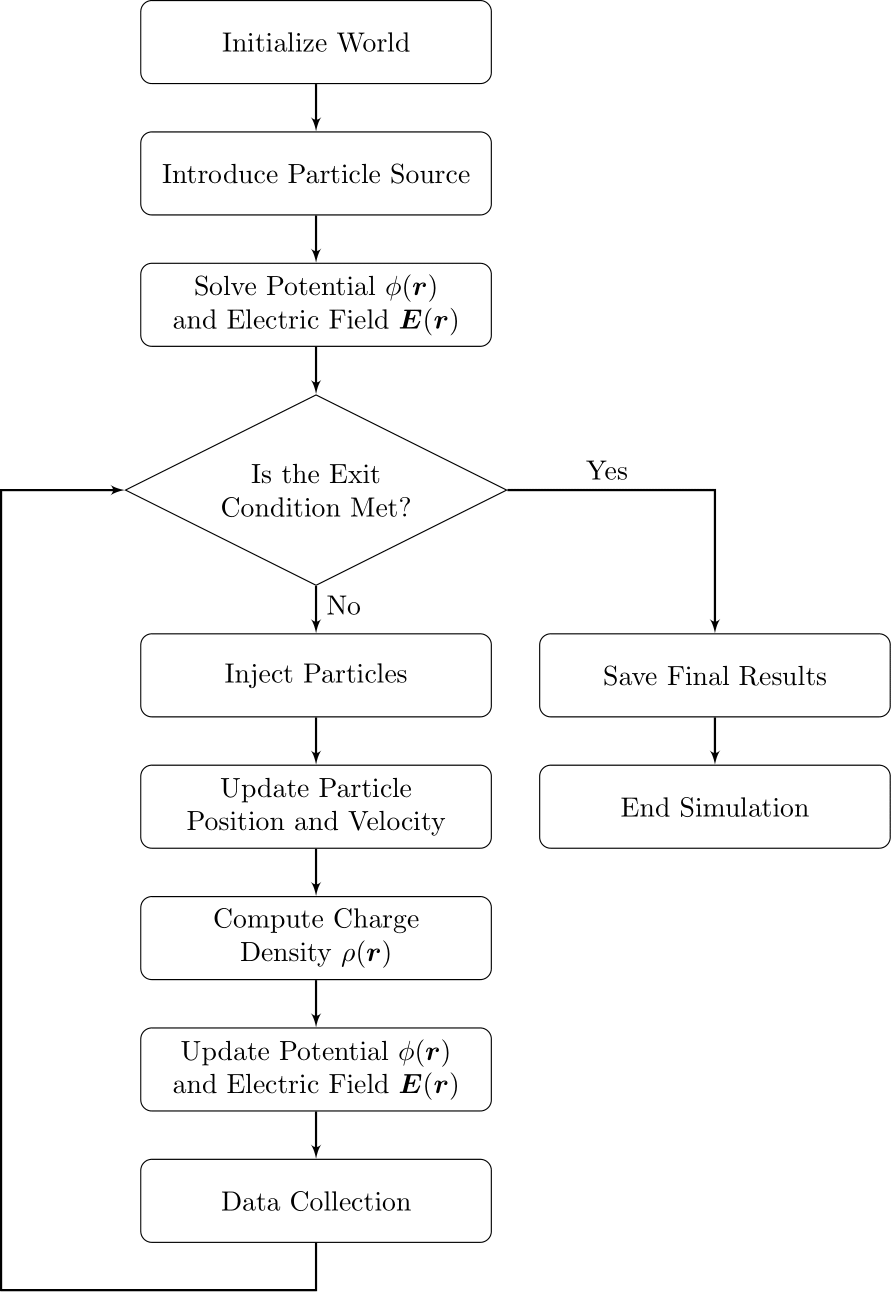
\includegraphics[width=0.65\linewidth]{figures/chapter 2/Flowchart_Studienprojekt with rho.png}
    \caption{Representation of the iterative Particle-in-Cell (\acs{PIC}) simulation process.}
    \label{fig: Flowchart}
\end{figure}

The Particle-in-Cell (\acs{PIC}) scheme employed in this research begins by initializing the discrete simulation domain and introducing the relevant particles. The initial charge and current densities are used to calculate the fields, which in turn enable the movement of particles (outlined in Section \ref{Sec: Particle Motion}). The fields are recalculated at each iteration based on the particles' updated positions and velocities. For simplicity, inter-particle collisions are not considered in this model. However, methods such as Monte Carlo Collisions (\acs{MCC}) and Direct Simulation Monte Carlo (\acs{DSMC}) can be implemented to account for these effects \cite{brieda_plasma_2019,birdsall_particle--cell_1991}. Furthermore, particles that exit the computational domain are either removed or reflected back, depending on the specific requirements of the simulation.

Practical plasma systems typically involve such an immense number of particles that simulating each particle individually becomes computationally impractical \cite{brieda_plasma_2019}. To address this, macroparticles are employed, each of which represents a large number of real particles. Each simulation particle is assigned a constant macroparticle weight $w_\mathrm{mp}$, which represents the number of real ions, electrons, or atoms it corresponds to. Each macroparticle can be envisioned as a cluster of $w_\mathrm{mp}$ real ions or electrons, all moving together with a shared position $\boldvec{x}_\mathrm{mp}$ and momentum $\boldvec{p}_\mathrm{mp}$ \cite{wu_particle--cell_2018}. Given that macroparticle weighting has no impact on the charge-to-mass ratio, the representative simulation particle moves along the same trajectory as the \textit{real} plasma particle.

\begin{equation}
    w_\mathrm{mp} = \frac{N_\mathrm{real}}{M_\mathrm{sim}}
\end{equation}


%\section{Discretize World Domain}

\section{Potential Solver}\label{Sec: potential solver}

To solve partial differential equations (\acs{PDE}s) like Poisson’s Equation in complex systems, numerical techniques such as finite difference methods (\acs{FDM}), finite element methods (\acs{FEM}), and spectral methods are essential \cite{brieda_plasma_2019}. Due to its relatively straightforward integration, \acs{FDM} was selected for the scope of the outlined simulation. This method builds upon the generally infinite Taylor Series expansion to approximate derivatives by replacing them with finite differences on a discrete grid. The Taylor Series expansion allows for estimating a function's value at a point offset by a small distance $\Delta x$ from another point. In one-dimensional cases, the equation can be typically expressed as \cite{arfken_mathematical_2013}:

\begin{equation}
f(x + \Delta x) = \sum_{n=0}^{\infty} \frac{(\Delta x)^n}{n!} f^{(n)}(x)
\end{equation}

Introducing the simplified notation $f_\mathrm{i} \equiv f(x_\mathrm{i})$ streamlines the handling of discrete node points $i$ in subsequent calculations. Correspondingly, the function values at adjacent nodes are given by $f_\mathrm{i+1} \equiv f(x + \Delta x)$ and $f_\mathrm{i-1} \equiv f(x - \Delta x)$. Given that $\Delta x \ll 1$ and due to the rapid factorial growth in the denominator, higher-order terms diminish quickly, leading to the following simplified expansion of the Taylor series \cite{brieda_plasma_2019}:


\begin{align}
\label{Eq: Taylor i+1}f_{\mathrm{i+1}} &= f_{\mathrm{i}} + \frac{\Delta x}{1!}\frac{\partial f}{\partial x} + \frac{(\Delta x)^2}{2!}\frac{\partial^2 f}{\partial x^2} + \frac{(\Delta x)^3}{3!}\frac{\partial^3 f}{\partial x^3} + \cdots\\
\nonumber\\\vspace{-2.5cm}
\label{Eq: Taylor i-1}f_{\mathrm{i-1}} &= f_{\mathrm{i}} - \frac{\Delta x}{1!}\frac{\partial f}{\partial x} + \frac{(\Delta x)^2}{2!}\frac{\partial^2 f}{\partial x^2} - \frac{(\Delta x)^3}{3!}\frac{\partial^3 f}{\partial x^3} + \cdots
\end{align}

A simplified equation with second-order accuracy can be derived by forming the sum of these two Taylor series expansions. The higher-order terms are denoted as \acs{HOT} but can be disregarded for the subsequent analyses:
\begin{align}    
f_{\mathrm{i+1}} + f_{\mathrm{i-1}} = 2 f_{\mathrm{i}} + (\Delta x)^2 \frac{\partial^2 f}{\partial x^2} + \text{HOT}
\end{align}
This expression can be rearranged to obtain the standard central difference formula for the second derivative:
\begin{align}
\frac{\partial^2 f}{\partial x^2} = \frac{f_\mathrm{i-1} - 2f_\mathrm{i} + f_\mathrm{i+1}}{(\Delta x^2)}
\end{align}

Substituting the Poisson Equation (see Eq. \ref{Eq: Poissions}) into this expression yields the discretized form of the second derivative of the electric potential $\phi$:

\begin{equation}\label{Eq: Discrete Poisson}
\frac{\phi_{\mathrm{i-1}} - 2\phi_{\mathrm{i}} + \phi_{\mathrm{i+1}}}{(\Delta x)^2} = -\frac{\rho_{\mathrm{i}}}{\epsilon_0} \quad\quad i \in [1, n_\mathrm{i} - 2]
\end{equation}

Generally, The system consists of a total of $n_\mathrm{i}$ nodes. However, the equation is not directly solvable at the boundaries, necessitating the use of Dirichlet boundary conditions. To clarify this one-dimensional derivation, the boundary values at the two edge nodes are fixed to $\phi_\mathrm{left}$ and $\phi_\mathrm{right}$, respectively. As a result, $n_\mathrm{i} -2$ equations remain to be solved for the inner nodes.

To demonstrate the \acs{FDM} approach for solving Poisson's equation, a mesh comprising a total of 5 nodes is employed as an illustrative example:
\begin{align}
    \phi_0 &= \phi_{\text{left}} \\
    (1 / \Delta x^2)(\phi_0 - 2\phi_1 + \phi_2) &= -\rho_1 / \epsilon_1 \\
    (1 / \Delta x^2)(\phi_1 - 2\phi_2 + \phi_3) &= -\rho_2 / \epsilon_2 \\
    (1 / \Delta x^2)(\phi_2 - 2\phi_3 + \phi_4) &= -\rho_3 / \epsilon_3 \\
    \phi_4 &= \phi_{\text{right}}
\end{align}

\begin{figure}[H]
    \centering
    \begin{tikzpicture}[scale = 1.8]
    % Define color
    %\definecolor{jlublau}{rgb}{0.0, 0.44, 0.87}

    % Set the spacing between points
    \def\spacing{1.4}
    \def\height{.3}
    % Draw vertical lines at the first and last points
    \draw[line,line width = 2pt] (0,-\height) --(0,\height);
    \draw[line,line width = 2pt] (4*\spacing,-\height) --(4*\spacing,\height);

    % Draw dashed lines between the points
    \draw[dashed] (0,0) -- (4*\spacing,0);
    
    % Loop to create 5 points and connect them with dashed lines
    \foreach \x in {0,1,...,4} {
        \fill[fill=jlublau, draw=black]  (\x*\spacing,0) circle (2.3pt);  % Draw blue points
        \node[above] at (\x*\spacing,\height) {$i=\x$}; % Add labels above each point
    }
    \fill[thmgreen,draw=black] (1.6*\spacing,0) circle (4.05pt);  % Red particle with radius 3pt

    \draw[-latex,thick] (-0.15, -0.42)-- (-0.03,-.12);  
    \node[below] at (-0.15, -0.36) {$\phi_\mathrm{left}$};
    % Arrow and label for the right side
    \draw[-latex,thick] (5.75, -0.42)-- (5.63,-.12);  
    \node[below] at (5.75, -0.36) {$\phi_\mathrm{right}$};

    

    \end{tikzpicture}
    \caption{Illustration of a one-dimensional mesh with a total of $n_\mathrm{i}=5$ nodes. The outer two nodes are constrained by Dirichlet boundary conditions to specific values of $\phi$}
    \label{fig:points}
\end{figure}

Furthermore, the discrete Poisson equation (see Eq. \ref{Eq: Discrete Poisson})  can be reformulated into matrix notation featuring a $n_\mathrm{i} \times n_\mathrm{i}$ coefficient matrix. Using the boundary conditions $\phi_\mathrm{left}$ and $\phi_\mathrm{right}$ from the previous example lead to the following expression:

\begin{equation}\label{Eq: Poisson Matrix}
    \frac{1}{(\Delta x)^2}
    \begin{pmatrix}
        (\Delta x)^2 & 0 & 0 & \dots & 0 \\
        1 & -2 & 1 & \dots & 0 \\
        \vdots & \ddots & \ddots & \ddots & \vdots \\
        0 & \dots & 1 & -2 & 1 \\
        0 & \dots & 0 & 0 & (\Delta x)^2
    \end{pmatrix}
    \begin{pmatrix}
        \phi(x_0) \\
        \phi(x_1) \\
        \vdots \\
        \phi(x_{n-2}) \\
        \phi(x_{n-1})
    \end{pmatrix}
    =
    \begin{pmatrix}
        \phi_\mathrm{left} \\
        \frac{\rho(x_1)}{\epsilon_0} \\
        \vdots \\
        \frac{\rho(x_{n-2})}{\epsilon_0} \\
        \phi_\mathrm{right}
    \end{pmatrix}
\end{equation}
\vspace{0.3cm}

Consequently, the problem shifts from solving a differential equation to solving a system of linear equations in the form:

\begin{equation}\label{Eq: general linear system}
    \boldvec{A} \boldvec{\phi} = \boldvec{b}
\end{equation}

Such a system can be solved either using direct methods or by employing iterative solving algorithms. 
Direct methods, such as the Thomas algorithm, always require a total of $2N$ computations for a system with $N$ unknowns, whereas iterative methods are not constrained by a fixed number of computations \cite{brieda_plasma_2019}. While the Thomas algorithm offers a straightforward implementation for one-dimensional problems, it struggles with more complex higher-dimensional applications \cite{brieda_plasma_2019}. Therefore, iterative solvers are employed for the field-solving scheme in this \acs{PIC} simulation, progressively refining the estimates for $\phi$ until a predefined convergence criterion is met (discussed in more detail in Section \ref{Sec: Convergence}).
\begin{comment}

\begin{align}
f(x+\Delta x) &= f(x) + \frac{\Delta x}{1!}\frac{\partial f}{\partial x} + \frac{(\Delta x)^2}{2!}\frac{\partial^2 f}{\partial x^2} + \frac{(\Delta x)^3}{3!}\frac{\partial^3 f}{\partial x^3} + \cdots\\
f(x-\Delta x) &= f(x) - \frac{\Delta x}{1!}\frac{\partial f}{\partial x} + \frac{(\Delta x)^2}{2!}\frac{\partial^2 f}{\partial x^2} - \frac{(\Delta x)^3}{3!}\frac{\partial^3 f}{\partial x^3} + \cdots
\end{align}


wegen boundary eigene Gleichung 
\end{comment}
\subsection{Gauss–Seidel Method}
\label{Sec: Gauss Seidel Method}
The Gauss-Seidel method is an iterative approach widely used for solving systems of linear equations, particularly when direct methods become computationally expensive. Similar to other iterative solvers, it starts with an initial guess for the solution vector and refines this guess at each step by progressively updating the variables until convergence is achieved \cite{sauer_numerical_2012}. In order to solve for all inner nodes $n$ in the system, the linear system of equations (see Eq. \ref{Eq: general linear system}) can be expanded into the following expression:

\begin{equation}
\begin{pmatrix}
a_{11} & \cdots & a_{1 \mathrm{n}}\\
\vdots & \ddots & \vdots\\
a_{\mathrm{n}1} & \cdots & a_{\mathrm{nn}}
\end{pmatrix}
\begin{pmatrix}
\phi_1 \\
\vdots\\
\phi_n
\end{pmatrix}
=
\begin{pmatrix}
b_1 \\
\vdots\\
b_n
\end{pmatrix}
\end{equation}

To exemplify, the matrix system can be expressed explicitly for a single component $b_\mathrm{i}$ as follows:

\begin{equation}
    b_\mathrm{i} = a_{\mathrm{i}1} \phi_1 + a_{\mathrm{i}2} \phi_2 + \dots + a_{\mathrm{ii}} \phi_i + \dots + a_{\mathrm{in}} \phi_n  
\end{equation}

Transforming the equation into a generalized form, it can be rearranged for the electric potential $\phi_\mathrm{i}$ at a single representative node $i$. In this form, the Kronecker delta $\delta_\mathrm{ij}$ is used to exclude the terms on the main diagonal from the total summation over all other nodes:

\begin{equation}
    \phi_\mathrm{i} = \frac{1}{a_{ii}} \left( b_\mathrm{i} - \sum_{j=1}^n (1-\delta_\mathrm{ij}) a_{\mathrm{{ij}}} \phi_\mathrm{j} \right)
\end{equation}

By introducing the counter variable $m$, the method iteratively updates the solution at each step ($m+1$). Incorporating the Poisson equation (see Eq. \ref{Eq: Poisson Matrix}) into this iterative framework leads to the following update formula for $ \phi_\mathrm{i}^{\mathrm{m+1}}$:
\begin{equation}
    \phi_\mathrm{i}^{\mathrm{m+1}} = -\frac{(\Delta x)^2}{2} \left[ b_\mathrm{i} - \left(  \frac{1}{(\Delta x)^2} \phi_\mathrm{i-1}^{\mathrm{m}} + \frac{1}{(\Delta x)^2} \phi_\mathrm{i+1}^{\mathrm{m}}\right)\right]
\end{equation}

The system can be significantly simplified since all non-boundary coefficients in Poisson's equation are identical. By rearranging the terms, the final form of the so-called Jacobi algorithm can be derived:

\begin{equation}
    \phi_i^{(m+1)} = \frac{\phi_{i-1}^{(m)} + \phi_{i+1}^{(m)} - b_\mathrm{i} (\Delta x)^2}{2} \quad \quad \text{with  }b_\mathrm{i}=-\frac{\rho_\mathrm{i}}{\epsilon_0}
\end{equation}

Building on that iterative framework, the Gauss-Seidel method offers an enhancement over the Jacobi approach, typically providing faster convergence rates \cite{brieda_plasma_2019}. The Gauss-Seidel (\acs{GS}) scheme always updates $\phi$ using the current values, whereas Jacobi completes an entire iteration using information from the previous step. This makes \acs{GS} more memory efficient, as it only needs to store one array instead of two. In contrast, the Jacobi method requires one array for the old values and another for the updated ones. This can be easily implemented using the following equation:
\begin{equation}
    \phi_i^{(m+1)} = \frac{\phi_{i-1}^{(m+1)} + \phi_{i+1}^{(m)} - b_\mathrm{i} (\Delta x)^2}{2}
\end{equation}

Since the $\phi_{i-1}^{(m+1)}$ node has already been calculated in the iteration loop, it is logical to directly incorporate it into the updated iteration step for $\phi_i^{(m+1)}$. This allows for more efficient computation by using the most recently updated values as soon as they become available.


\subsection{Successive Over-Relaxation}

To further speed up the convergence rate, a commonly used approach is the implementation of Successive Over-Relaxation (\acs{SOR}). This method refines the Gauss-Seidel approach by introducing a relaxation factor $w$, accelerating the updates to $\phi$ by making each iteration step more aggressive. Furthermore, for values of $w$ between 0 and 1, known as under-relaxation, the method can help achieve successful convergence in systems that might otherwise diverge using the conventional Gauss-Seidel method \cite{allahviranloo_successive_2005}. When $w > 1$, the convergence rate is accelerated, with a typical range for $w$ being between 1 and 2. In applications such as electrostatic \acs{PIC} simulations, a commonly used value is around 1.4, as it balances faster convergence speeds with reliable outcomes \cite{brieda_plasma_2019}. However, the ideal value of $w$ is highly dependent on the specific characteristics of the system and must be determined empirically through trial and error (discussed in depth in Section \ref{Sec: Optimizing Relaxation Factor}). Generally, the updated potential is determined as follows:

\begin{equation}
\phi_\mathrm{updated} = \phi_\mathrm{old} + w (\phi_\mathrm{new} - \phi_\mathrm{old})
\end{equation}


\subsection{Convergence}\label{Sec: Convergence}

In iterative methods, convergence refers to the process of obtaining progressively closer approximations to the solution of a system with each iteration \cite{barrett_templates_1994}. Generally, the process begins with an initial guess for the variable of interest $\phi$ and refines it through successive iterations, ideally converging to the true solution. Stationary methods, such as the introduced Gauss-Seidel method (see Section \ref{Sec: Gauss Seidel Method}), follow this approach to progressively reduce the error in each iteration \cite{barrett_templates_1994}. Convergence is achieved when the difference between iterations diminishes, ideally approaching zero as the iteration step $m$ increases, and the solution stabilizes. Mathematically, this can be expressed as:

\begin{equation}
    \boldsymbol{\phi} = \lim_{m \to \infty} \boldsymbol{\phi}^{m}
\end{equation}


In practical applications, an error margin is introduced with $\boldvec{R}$ representing the residual, which measures the discrepancy in the system at each iteration. As $\phi^\mathrm{m}$ approaches the true solution, $R^\mathrm{m}$ becomes progressively smaller, indicating that the solution is converging. This relationship can be represented by the following equation \cite{brieda_plasma_2019}:
\begin{align}
    \boldvec{A} \boldvec{\phi}^\mathrm{m} &= \boldvec{b}^\mathrm{m} + \boldvec{R}^\mathrm{m}\\ 
    \intertext{The magnitude of the residual vector is defined using the $L_2$ norm, as shown in the following equation \cite{brieda_plasma_2019}:}
    \|R\| &= \sqrt{\frac{\sum_{i}^{n} (R_i)^2}{n}}\\
    \intertext{In the multidimensional simulation outlined in this report, this calculation is performed every 25 iterations due to the significant computational demands involved. The stopping criteria are based on either reaching a maximum number of iterations or the residual falling below a predefined error threshold:}
     \|R\| &< \epsilon_\mathrm{tol}
\end{align}


\begin{comment}


\begin{equation}
    \phi = \lim_{m \to \infty} \phi^m \quad \text{such that} \quad |\phi^{m+1} - \phi^m| < \epsilon
\end{equation}
\end{comment}
\section{Electric Field Solver}
The accurate calculation of the Lorentz force, which governs the movement of charged particles, requires determining the electric field at each computational node. Generally, the electric field is determined by the gradient of the electric potential (see Eq. \ref{E to Phi}). In the one-dimensional case, this relationship simplifies to the derivative of $\phi$ with respect to $x$, as shown in the following equation:

\begin{equation}
E = -\frac{\partial \phi}{\partial x}
\end{equation}

Using the Taylor series expansion once again for the adjacent nodes $i+1$ (see Eq. \ref{Eq: Taylor i+1}) and  $i-1$ (see Eq. \ref{Eq: Taylor i-1}), the resulting expression can be obtained:

\begin{equation}
    f_{i+1} - f_{i-1} = 2\Delta x \frac{\partial f}{\partial x} + \text{HOT}
\end{equation}

This expression can be rearranged to approximate the first derivative using the standard central-difference formula as:

\begin{equation}\label{Eq: Electric field 1d central}
    \frac{\partial f}{\partial x} \approx \frac{f_{i+1} - f_{i-1}}{2\Delta x}
\end{equation}

This approximation is second-order accurate, but since it involves both $i+1$ and $i-1$ terms, it can only be applied to internal nodes. For Boundary nodes we can use Equation \ref{Eq: Taylor i+1} and Equation \ref{Eq: Taylor i-1} directly discarding the second derivative term. However, those terms are only first order accurate leading to a higher innacurary at the boundary compared to the inner nodes. Alternativly, we can introduce the equivalent Taylor series for the estimate value at $i+2$ or respectively $i-2$:
\begin{align}
    f_{i+2} &= f_i + (2\Delta x) \frac{\partial f}{\partial x} + \frac{(2\Delta x)^2}{2} \frac{\partial^2 f}{\partial x^2} \\
    f_{i-2} &= f_i - (2\Delta x) \frac{\partial f}{\partial x} + \frac{(2\Delta x)^2}{2} \frac{\partial^2 f}{\partial x^2}
\end{align}

A mathematically useful approach is to subtract Equation \ref{Eq: Taylor i+1} four times:
\begin{align}
      f_{i+2} - 4 f_{i+1} &=  f_i + (2\Delta x) \frac{\partial f}{\partial x} + 2(\Delta x)^2\frac{\partial^2 f}{\partial x} - 4 f_i -4 \Delta x\frac{\partial f}{\partial x} - \frac{4 (\Delta x)^2}{2} \frac{\partial^2 f}{\partial x^2}\nonumber\\
      &= -3 f_i - 2 \Delta x \frac{\partial f}{\partial x} \\
      \intertext{This results in a second-order accurate expression for the solution at the starting boundary:}
      \text{Forward:} \quad \quad \frac{\partial f}{\partial x} &\approx \frac{-3f_i + 4f_{i+1} - f_{i+2}}{2\Delta x}\\
      \intertext{Using the same approach for the Taylor expansion at the node $i- 2$ and subtracting Equation \ref{Eq: Taylor i-1} four times leads to the solution at the outermost node:}
      \text{Backward:}\quad \quad \frac{\partial f}{\partial x} &\approx \frac{f_{i-2} - 4f_{i-1} + 3f_i}{2\Delta x}
\end{align}

To make \acs{ES PIC} simulations applicable for practical scenarios, it is necessary to implement the electric field solver in three dimensions. For this purpose, the nabla operator ($\nabla$) is employed to cover all three spatial dimensions, providing a comprehensive expression for the electric field in 3D:
\begin{align}
    \boldvec{E} =  -\left( \frac{\partial \phi}{\partial x} \hat{e}_1 + \frac{\partial \phi}{\partial y} \hat{e}_2 + \frac{\partial \phi}{\partial z} \hat{e}_3 \right)
\end{align}

By incorporating Equation \ref{Eq: Electric field 1d central}, the electric field components can be expressed using the central difference scheme for each spatial direction. Here, the counting variables $i$, $j$, and $k$ correspond to the discretized grid points in the $x$-, $y$-, and $z$-dimension, respectively. This leads to the detailed expression shown below:

\begin{align}
    \boldvec{E} = \left( \frac{\phi_\mathrm{i-1,j,k} - \phi_\mathrm{i+1,j,k}}{2\Delta x} \right) \hat{e}_1 + \left( \frac{\phi_\mathrm{i,j-1,k} - \phi_\mathrm{i,j+1,k}}{2\Delta y} \right) \hat{e}_2 + \left( \frac{\phi_\mathrm{i,j,k-1} - \phi_\mathrm{i,j,k+1}}{2\Delta z} \right) \hat{e}_3
\end{align}

Exemplarily, the boundary nodes in the $x$-dimension with a total of $n_\mathrm{i}$ nodes can be calculated as follows:
\begin{align}
\text{Forward:}&\quad\quad\left( E_\mathrm{x} \right)_\mathrm{i = \mathrm{0}} = \frac{3\phi_\mathrm{\mathrm{0}, j, k} + 4\phi_\mathrm{\mathrm{1}, j, k} - \phi_\mathrm{\mathrm{2}, j, k}}{2\Delta x}\\
\text{Backward:}&\quad\quad    \left( E_\mathrm{x} \right)_\mathrm{i = n_\mathrm{i}-1} = \frac{-\phi_\mathrm{n_\mathrm{i}-3, j, k} + 4\phi_\mathrm{n_\mathrm{i}-2, j, k} - \phi_\mathrm{n_\mathrm{i}-1, j, k}}{2\Delta x}
\end{align}


\begin{comment}

\begin{align}
    f_{i-2} - 4f_{i-1} &= f_i + (2\Delta x)\frac{\partial f}{\partial x} + 2(\Delta x)^2 \frac{\partial^2 f}{\partial x^2} - 4f_i - 4\Delta x \frac{\partial f}{\partial x} - \frac{4(\Delta x)^2}{2} \frac{\partial^2 f}{\partial x^2}\\
    &= -3f_i + 2\Delta x \frac{\partial f}{\partial x}\\
    \intertext{Umstellen der Gleichung führt zu:}
\end{align}


We use again taylor expansion for any function:
\begin{align}
f_{i+1} &= f_i + \frac{\Delta x}{1} \frac{\partial f}{\partial x} + \frac{(\Delta x)^2}{2} \frac{\partial^2 f}{\partial x^2} + \text{HOT}\\
f_{i-1} &= f_i - \frac{\Delta x}{1} \frac{\partial f}{\partial x} + \frac{(\Delta x)^2}{2} \frac{\partial^2 f}{\partial x^2} + \text{HOT}
\end{align}



\begin{align}
    \text{Forward:}  \quad\quad \frac{\partial f}{\partial x} &\approx \frac{f_{i+1} - f_i}{\Delta x}\\
    \text{Backward:}  \quad\quad\frac{\partial f}{\partial x} &\approx \frac{f_i - f_{i-1}}{\Delta x}
\end{align}



Actually dont have to write Equations again down just ref via \ref{Eq: Taylor i+1} for i+1 and \ref{Eq: Taylor i-1} for i-1
we subtract the second equation from the first. This gives us

- Unterscheiden zwischen:\\
1. linker node -> forward\\
2. Rechter noder -> backward\\ 
3. Central node -> normal\\

\end{comment}
\section{Particle Mover}
\label{Sec: Particle Motion}


In particle-based simulations, such as Particle-In-Cell (\acs{PIC}) methods, particles are characterized by their mass, charge, position, and velocity. To model their dynamics, it is essential to solve Newton's equations of motion over a long period, starting from a set of predefined initial conditions \cite{young_leapfrog_2013}. Since time advances unidirectionally, techniques like central difference methods used for spatial problems are not applicable for time integration \cite{brieda_plasma_2019}. Generally, this type of integration with the discrete time step $\Delta t$ can be expressed as follows:
 \begin{align}
\boldvec{x}^{\mathrm{k+1}} &= \boldvec{x}^{\mathrm{k}} + \boldvec{v}^{\mathrm{k}} \Delta t, \\
\boldvec{v}^{\mathrm{k+1}} &= \boldvec{v}^{\mathrm{k}} + \frac{q \boldvec{E}^{\mathrm{k}}}{m}  \Delta t
\end{align}

This approach is known as the Forward Euler method, a first-order accurate technique that requires initial conditions for the velocity $v$ and the position $x$ \cite{brieda_plasma_2019}. As an explicit method, it calculates the next iteration step, $k+1$, solely based on the information available at the current step, $k$.


\subsection{Leapfrog Method}
Methods such as the Euler method typically require the time step $\Delta t$ to approach zero in order to converge to an accurate solution \cite{brieda_plasma_2019}. This restriction results in extremely high computational costs, making practical implementation difficult. To address these limitations, the leapfrog method is a commonly used algorithm due to its relatively simple usage and improved accuracy. The leapfrog method takes advantage of the midpoint method, a frequently employed technique in numerical differentiation and integration. By interpolating the velocity with an additional half-step at the beginning, this method achieves second-order accuracy:
\begin{align}
        \boldvec{x}^\mathrm{k+1} &= \boldvec{x}^\mathrm{k} + \left(\frac{\boldvec{v}^\mathrm{k} + \boldvec{v}^\mathrm{k+1}}{2}\right) \Delta t\\
        \frac{\boldvec{v}^\mathrm{k} + \boldvec{v}^\mathrm{k+1}}{2} &= \boldvec{v}^\mathrm{k} + \frac{q\,\boldvec{E}^\mathrm{k}}{ m}\ \frac{\Delta t}{2}\equiv \boldvec{v}^\mathrm{k+0.5}
\end{align}


The values for position and velocity are calculated in an alternating manner, where velocities are known at half time steps ($k=-0.5,0.5,1.5,...$) and particle positions are known at full time steps  ($k=0,1,2,...$). This staggered approach characterizes the leapfrog method as symplectic, helping to preserve the system's energy and ensuring 'global stability' in long-term simulations.

\begin{figure}[H]
    \centering
    \begin{tikzpicture}
    \def\yshift{-0.6}

    % Time axis
    \draw[-latex,line width = 1.5pt] (0,0) -- (11,0) node[anchor=west] {$t$};

    % Time markers
    \foreach \x/\xtext in {0/, 2/, 4/, 6/, 8/, 10/}
      \draw (\x cm,3pt) -- (\x cm,-3pt) node[anchor=north] {\xtext};

    \def\ydash{-1.9}
    
    \foreach \x/\xtext in {0/$t_{-1/2}$, 4/$t_{1/2}$, 8/$t_{3/2}$}
      \draw[dashed] (\x cm,\ydash) -- (\x cm,-0.7) node[anchor=north] {};
    %\draw[dashed] (0,-.7) -- (0,-1.9);

    % Labels for fractional times, moved down
    \node[below] at (0,\ydash) {$t_{-1/2}$};
    \node[below] at (4,\ydash) {$t_{1/2}$};
    \node[below] at (8,\ydash) {$t_{3/2}$};

        \foreach \x/\xtext in {2/$t_0$,6/$t_1$,10/$t_2$}
      \draw[dashed] (\x cm,\ydash) -- (\x cm,-0.23) node[anchor=north] {};

    % Labels for fractional times, moved down
    \node[below] at (2,\ydash) {$t_{0}$};
    \node[below] at (6,\ydash) {$t_{1}$};
    \node[below] at (10,\ydash) {$t_{2}$};

    \colorlet{darkjlublue}{jlublau!90!black}

    % Define a scaling factor for the line width
    \def\thicknessFactor{1.5pt} 
    % Blue arrows (v_-1/2, v_1/2, v_3/2) in darkjlublue color
    \draw[-latex,darkjlublue,line width = \thicknessFactor] (0,0+\yshift) .. controls (0.5,-1.3+\yshift) and (3.5,-1.3+\yshift) .. (3.9,0+\yshift) node[midway,below] ;
    \draw[-latex,darkjlublue,line width = \thicknessFactor] (4,0+\yshift) .. controls (4.5,-1.3+\yshift) and (7.5,-1.3+\yshift) .. (7.9,0+\yshift) node[midway,below] ;
    \draw[-latex,darkjlublue,line width = \thicknessFactor] (8,0+\yshift) .. controls (8.5,-1.3+\yshift) and (11.5,-1.3+\yshift) .. (11.9,0+\yshift) node[midway,below];
    
    \def\yshift_v{-0.1}
    % Nodes with text under the specified points in darkjlublue color with bold font
    \node[below,darkjlublue] at (0, +\yshift_v) {\bfseries $v_{-1/2}$};
    \node[below,darkjlublue] at (4, +\yshift_v) {\bfseries $v_{1/2}$};
    \node[below,darkjlublue] at (8, +\yshift_v) {\bfseries $v_{3/2}$};

    \colorlet{darkthmgreen}{thmgreen!90!black}

    \def\yshift_x{-0.1}
    % Nodes with text under the specified points in darkjlublue color with bold font
    \node[above,darkthmgreen] at (2, -\yshift_x) {\bfseries $x_0$};
    \node[above,darkthmgreen] at (6, -\yshift_x) {\bfseries $x_1$};
    \node[above,darkthmgreen] at (10, -\yshift_x) {\bfseries $x_2$};

    
    \def\thicknessFactor{1.5pt} 
    \def\yshift{-0.6}
    \draw[-latex,darkthmgreen,line width = \thicknessFactor] (2,0-\yshift) .. controls (2.5,1.3-\yshift) and (5.5,1.3-\yshift) .. (5.9,0-\yshift) node[midway,below] ;
    \draw[-latex,darkthmgreen,line width = \thicknessFactor] (6,0-\yshift) .. controls (6.5,1.3-\yshift) and (9.5,1.3-\yshift) .. (9.9,0-\yshift) node[midway,below] ;


    %\draw[latex-,red,line width = \thicknessFactor] (0,0+.3) .. controls (0.5,1.3-\yshift) and (1.5,1.3-\yshift) .. (1.9,0-\yshift);

%    \node[above,red] at (1, 2) {\bfseries $test$};





    
    \end{tikzpicture}
    \caption{Illustration of the leapfrog method, showing the alternating calculation of particle positions ($x_\mathrm{n}$) and velocities ($v_\mathrm{n-1/2}$) at staggered time steps.}
    \label{fig:enter-label}
\end{figure}

To initialize the leapfrog method, a velocity rewind for injected particles by half a time step is necessary. This is achieved by interpolating the initial velocity values $v^0$ with the previously calculated electric field $\boldvec{E}^0$, as shown in the equation below:
\begin{equation}
    \boldvec{v}^\mathrm{-0.5} = \boldvec{v}^\mathrm{0} -  \frac{q\,\boldvec{E}^\mathrm{0}}{ m}\ \frac{\Delta t}{2}
\end{equation}



\subsection{Interpolation}
As previously discussed, the electric field is only defined at the discrete nodes of the computational mesh. However, to obtain numerically stable and physically meaningful results, it is crucial to evaluate the electric field at the position of each particle within its corresponding cell \cite{brieda_plasma_2019}. To achieve this, the electric field at the surrounding grid nodes is linearly interpolated by employing a normalized parameter $d_\mathrm{i} \in [0, 1]$. For a total of $D$ spatial dimensions, there must be a corresponding parameter for each dimension to weight the contributions of the $2^\mathrm{N}$ neighboring nodes. For the one-dimensional case, the electric field at the particle location $x_\mathrm{i}+d_\mathrm{i}$ can be accurately approximated as follows:
\begin{align}
    E &= E_\mathrm{i} + d_\mathrm{i}\left(E_\mathrm{i+1} - E_\mathrm{i}\right)\\
    E &=  \left( 1-d_\mathrm{i}\right)E_\mathrm{i} + d_\mathrm{i}E_\mathrm{i+1}
\end{align}

This gathering operation enables the use of multiple mesh-based values to evaluate particle-related properties at a specific location \cite{brieda_plasma_2019}. The interpolated field values are then used to update the particle's velocity and position using the previously discussed leapfrog method.

\begin{figure}[H]
    \centering
\begin{tikzpicture}[scale=.8]

\def\thickness{1.3}

% Axis
\draw[-latex,line width = 1.1] (0,0) -- (12,0) node[anchor=north] {$x$};
\draw[-latex,line width = 1.1] (0,0) -- (0,6.5) node[anchor=east] {$E(x)$};

% Function line
\draw[line width = \thickness] (2,1.7) -- (9,4.4);
\draw[line width = \thickness] (.8,0) -- (2,1.7);
\draw[line width = \thickness] (9,4.4) -- (11.2,4.6);

% Dashed lines for points
\draw[dashed,thick] (2,0) -- (2,1.7);
\draw[dashed,thick] (2,1.7) -- (0,1.7);

\draw[dashed,thick] (6.5,3.45)  -- (6.5,0);
\draw[dashed,thick] (6.5,3.45)  -- (0,3.45);

\draw[dashed,thick] (9,4.4)  -- (9,0);
\draw[dashed,thick] (9,4.4)  -- (0,4.4);

\def\thicknessaxis{1.1}
% Ticks and labels on axes
\draw[line width = \thicknessaxis] (2,0) -- (2,-0.2) node[anchor=north] {$x_\mathrm{i}$};
\draw[line width = \thicknessaxis] (6.5,0) -- (6.5,-0.2) node[anchor=north] {$x_\mathrm{i}+d_\mathrm{i}$};
\draw[line width = \thicknessaxis] (9,0) -- (9,-0.2) node[anchor=north] {$x_\mathrm{i+1}$}; 

\draw[line width = \thicknessaxis] (0,1.7) -- (-0.2,1.7) node[anchor=east] {$E(x_\mathrm{i})$}; 
\draw[line width = \thicknessaxis] (0,3.45) -- (-0.2,3.45) node[anchor=east] {$E(x_\mathrm{i}+d_\mathrm{i})$}; 
\draw[line width = \thicknessaxis] (0,4.4) -- (-0.2,4.4) node[anchor=east] {$E(x_\mathrm{i+1})$};
% Points
\filldraw[fill=white, draw=white] (2, 1.7) circle (2.3pt*2.2);
\fill[fill=jlublau, draw=black]  (2, 1.7) circle (2.3pt*2.2);  % Draw blue points
\filldraw[fill=white, draw=white] (9,4.4) circle (2.3pt*2.2);
\fill[fill=jlublau, draw=black]  (9,4.4) circle (2.3pt*2.2);  % Draw blue points
\fill[thmgreen,draw=black] (6.5,3.45) circle (4.05pt*2.2);  % Green particle

% Additional points
%\fill[fill=jlublau, draw=black]  (2, 7) circle (2.3pt*2.2);  % Draw blue points
%\fill[fill=jlublau, draw=black]  (9,7) circle (2.3pt*2.2);  % Draw blue points
%\fill[thmgreen,draw=black] (6.5,7) circle (4.05pt*2.2);  % Green particle

\end{tikzpicture}



    \caption{Visualization of the linear interpolation of the electric field values at the adjacent nodes $i$ and $i+1$ to estimate the field at the particle's position $x_\mathrm{i}+d_\mathrm{i}$.}
    \label{fig:enter-label}
\end{figure}

In contrast to gathering, the scattering process is used to distribute particle-based data back to the computational mesh. During this process, each macroparticle influences the surrounding mesh nodes by contributing to quantities such as the number density $n$. The number density is reset and recalculated at every iteration, based solely on the current positions of particles within each cell. In order to perform this calculation, the algorithm loops over all particles of different species, taking the node volume $V_\mathrm{node}$ into account:
\begin{align}
    n_\mathrm{i}^{\mathrm{new}} &= n_\mathrm{i}^{\mathrm{old}} +  (1 - d_\mathrm{i}) \frac{w_\mathrm{mp}}{V_\mathrm{node}}\\
    n_\mathrm{i+1}^{\mathrm{new}} &= n_\mathrm{i+1}^{\mathrm{old}} + d_\mathrm{i} \frac{w_\mathrm{mp}}{V_\mathrm{node}}
\end{align}
Lastly, the charge density $\rho$ is updated to be used in the next iteration step by the potential solver (discussed in section \ref{Sec: potential solver}). This density is reset to zero at each iteration before being incremented by the charge $q$ of each species, scaled by the previously introduced number density $n_\mathrm{i}^\mathrm{new}$:

\begin{equation}
\rho_\mathrm{i}^\mathrm{new} = \rho_\mathrm{i}^\mathrm{old} + q \cdot n_\mathrm{i}^\mathrm{new}
\end{equation}


\begin{comment}

 
Update the charge density to feed in the next iteration back to the potential solver

same for rho, gets reseted to zero every iteration


\begin{verbatim}
# velocity rewind
vel -= self.charge / self.mass * ef_part * (0.5 * self.world.get_dt())
\end{verbatim}

    \begin{figure}[H]
    \centering
    \begin{tikzpicture}
    \def\yshift{-0.6}

    % Time axis
    \draw[-latex,line width = 1.5pt] (0,0) -- (11,0) node[anchor=west] {$t$};

    % Time markers
    \foreach \x/\xtext in {0/, 2/, 4/, 6/, 8/, 10/}
      \draw (\x cm,3pt) -- (\x cm,-3pt) node[anchor=north] {\xtext};

    \def\ydash{-1.9}
    
    \foreach \x/\xtext in {0/$t_{1/2}$, 4/$t_{3/2}$, 8/$t_{5/2}$}
      \draw[dashed] (\x cm,\ydash) -- (\x cm,-0.7) node[anchor=north] {};
    %\draw[dashed] (0,-.7) -- (0,-1.9);

    % Labels for fractional times, moved down
    \node[below] at (0,\ydash) {$t_{1/2}$};
    \node[below] at (4,\ydash) {$t_{3/2}$};
    \node[below] at (8,\ydash) {$t_{5/2}$};

        \foreach \x/\xtext in {2/$t_1$,6/$t_2$,10/$t_3$}
      \draw[dashed] (\x cm,\ydash) -- (\x cm,-0.23) node[anchor=north] {};

    % Labels for fractional times, moved down
    \node[below] at (2,\ydash) {$t_{1}$};
    \node[below] at (6,\ydash) {$t_{2}$};
    \node[below] at (10,\ydash) {$t_{3}$};

    \colorlet{darkjlublue}{jlublau!90!black}

    % Define a scaling factor for the line width
    \def\thicknessFactor{1.5pt} 
    % Blue arrows (v_1/2, v_3/2, v_5/2) in darkjlublue color
    \draw[-latex,darkjlublue,line width = \thicknessFactor] (0,0+\yshift) .. controls (0.5,-1.3+\yshift) and (3.5,-1.3+\yshift) .. (3.9,0+\yshift) node[midway,below] ;
    \draw[-latex,darkjlublue,line width = \thicknessFactor] (4,0+\yshift) .. controls (4.5,-1.3+\yshift) and (7.5,-1.3+\yshift) .. (7.9,0+\yshift) node[midway,below] ;
    \draw[-latex,darkjlublue,line width = \thicknessFactor] (8,0+\yshift) .. controls (8.5,-1.3+\yshift) and (11.5,-1.3+\yshift) .. (11.9,0+\yshift) node[midway,below];
    
    \def\yshift_v{-0.1}
    % Nodes with text under the specified points in darkjlublue color with bold font
    \node[below,darkjlublue] at (0, +\yshift_v) {\bfseries $v_{1/2}$};
    \node[below,darkjlublue] at (4, +\yshift_v) {\bfseries $v_{3/2}$};
    \node[below,darkjlublue] at (8, +\yshift_v) {\bfseries $v_{5/2}$};

    \colorlet{darkthmgreen}{thmgreen!90!black}

    \def\yshift_x{-0.1}
    % Nodes with text under the specified points in darkjlublue color with bold font
    \node[above,darkthmgreen] at (2, -\yshift_x) {\bfseries $x_1$};
    \node[above,darkthmgreen] at (6, -\yshift_x) {\bfseries $x_2$};
    \node[above,darkthmgreen] at (10, -\yshift_x) {\bfseries $x_3$};

    
    \def\thicknessFactor{1.5pt} 
    \def\yshift{-0.6}
    \draw[-latex,darkthmgreen,line width = \thicknessFactor] (2,0-\yshift) .. controls (2.5,1.3-\yshift) and (5.5,1.3-\yshift) .. (5.9,0-\yshift) node[midway,below] ;
    \draw[-latex,darkthmgreen,line width = \thicknessFactor] (6,0-\yshift) .. controls (6.5,1.3-\yshift) and (9.5,1.3-\yshift) .. (9.9,0-\yshift) node[midway,below] ;



    
    \end{tikzpicture}
    \caption{Caption}
    \label{fig:enter-label}
\end{figure}

\end{comment}
\section{Introduction Particle Sources}

To simulate the flow of charged particles in a system, it is crucial to introduce these particles in a way that aligns with the specific problem being addressed. Generally, each particle contains distinct information about its position, velocity, and macroparticle weight $w_\mathrm{mp}$. Moreover, particles from the same gas species can be grouped to simplify the management of different ion and electron behaviors in the later stages of the simulation. For all particles within a given species, physical properties like mass and charge are uniform and need to be assigned only once during the initialization process. Although macroparticle weight can vary, particles of the same species tend to share the same weight, allowing for easier collective handling at the species level \cite{brieda_plasma_2019}. In general, the behavior of a local particle density $\rho$ across space and time is governed by the principle of mass conservation expressed mathematically through the use of the continuity equation \cite{griffiths_introduction_2017}:

\begin{align}
\frac{\partial \rho}{\partial t} &+ \nabla \cdot (\rho \boldvec{v}) = 0\\
    \intertext{By integrating over the computational volume and applying the Divergence Theorem on the right-hand side enables to rewrite the equation as follows \cite{brieda_plasma_2019}:}
    \int_V \frac{\partial \rho}{\partial t} dV &= - \int_V \nabla \cdot (\rho \boldvec{v}) dV \\
    &= - \oint_\mathrm{S} \rho \boldvec{v} \cdot \hat{e}_\mathrm{3} \, dA \\
    \intertext{Considering the initial state, where the density and velocity $\boldvec{v}_\mathrm{z}$ of the inflowing ions are assumed to be uniform across the entire integration surface, the rate of change in the number of particles $N$ over time can be expressed as:}
    \frac{dN}{dt} &= \rho v_\mathrm{z} A_{\text{inlet}}
\end{align}

This equation describes the number of real particles entering the system per time step through a single surface area $A_{\text{inlet}}$. The particles are assumed to have a unidirectional velocity component $\boldvec{v}_\mathrm{z}$, normal to this surface. The number of particles to inject per time step $\Delta t$ to maintain a consistent flow rate $\dot{N}$ can be thus calculated as:
\begin{equation}
    N = \dot{N} \Delta t
\end{equation}


\subsection{Cold Beam Source}

To simplify the simulation process, a cold beam source is selected as the particle injection method, which avoids the added complexities introduced by thermal motion \cite{brieda_plasma_2019}. Generally, particle velocity in a gas kinetic system typically comprises two main components. The drift velocity represents $\bar{v}_\mathrm{d}$ the collective, directed movement of particles, while the thermal velocity $\tilde{v}_\mathrm{th}$ accounts for the random distribution of velocities about the mean \cite{brieda_plasma_2019}. This can be mathematically expressed as:

\begin{equation}
    v = \bar{v}_\mathrm{d} + \tilde{v}_\mathrm{th}
\end{equation}

As the name suggests, the temperature of a cold beam source is assumed to be approximately zero, effectively eliminating the contribution of thermal velocity. With this assumption, the thermal velocity can be neglected, simplifying the velocity to consist solely of the drift component. Since all particles are assumed to have equal drift velocities in the context of the outlined simulation, the cold beam source injects a stream of mono-energetic particles into the system.

As previously discussed, the particles are injected into the simulation domain through a single injection surface $A_\mathrm{inlet}$. This area can be defined in a discretized form as follows:

\begin{equation}
    A_{\text{inlet}} = L_x L_y = (n_i - 1) \Delta x \cdot (n_j - 1) \Delta y
\end{equation}

To ensure that particles are evenly and realistically distributed across the injection plane, incorporating randomness into the simulation process is beneficial. This stochastic approach was implemented by the use of the variables $\mathcal{R}_1$ and $\mathcal{R}_2$, which represent uniformly distributed values between 0 and 1:

\begin{align}
    x &= x_0 + \mathcal{R}_1 L_\mathrm{x} \\
    y &= y_0 + \mathcal{R}_2 L_\mathrm{y} \\
    z &= z_0
\end{align}
The particle position $(x,y,z)$ can thus be defined relative to the origin coordinates $(x_0,y_0,z_0)$. The $x$ and $y$ coordinates are then scaled randomly by the total side length of the injection plane, $L_\mathrm{x}$ and $L_\mathrm{y}$, to place the particles across the full area of the injection plane. For a small set of particles, this process can be illustrated as follows:

\begin{figure}[H]
    \centering

\begin{tikzpicture}[scale=1.5, rotate around y=-22]

    % Front face (colored face that we are looking into)

    \draw[thick,-latex] (-3,-2,0) -- (-2.2,-2,0) node[anchor=north] {$z$};  % x-axis
    \draw[thick,-latex] (-3,-2,0) -- (-3,-1.2,0) node[anchor=west] {$y$};   % y-axis
    \draw[thick,-latex] (-3,-2,0) -- (-3,-2,-.8) node[anchor=north] {$x$};   % z-axis


    
    \fill[gray!50] (0,-1,-1) -- (0,1,-1) -- (0,1,1) -- (0,-1,1) -- cycle;
    \draw[thick] (0,-1,-1) -- (0,1,-1) -- (0,1,1) -- (0,-1,1) -- cycle;

    % Top face (extended x-direction to 6)
    \draw[thick,gray!60] (0,1,1) -- (5,1,1) -- (5,1,-1) -- (0,1,-1) -- cycle;

    % Bottom face (extended x-direction to 6)
    \draw[thick,gray!60] (0,-1,1) -- (5,-1,1) -- (5,-1,-1) -- (0,-1,-1) -- cycle;

    % Back face (extended x-direction to 6)
    \draw[thick,gray!60] (5,-1,1) -- (5,1,1) -- (5,1,-1) -- (5,-1,-1) -- cycle;

    % Left face (remains the same)
    \draw[thick,gray!60] (0,-1,1) -- (0,1,1) -- (5,1,1) -- (5,-1,1) -- cycle;

    % Right face (remains the same)
    \draw[thick,gray!60] (0,-1,-1) -- (0,1,-1) -- (5,1,-1) -- (5,-1,-1) -- cycle;
    \draw[thick] (0,-1,-1) -- (0,1,-1) -- (0,1,1) -- (0,-1,1) -- cycle;

    
    \draw [decorate,decoration={brace,amplitude=10pt,mirror,raise=5pt},thick] (0,-1,1) -- (5,-1,1) node[midway, under,xshift=-0.2em,yshift=-2em]{$L_z$};
    
    \draw [decorate,decoration={brace,amplitude=10pt,raise=5pt,rotate around y=90},thick,] (0,-1,1) -- (0,1,1) node[midway, under, xshift = -2.2em]{$L_y$};
    
\draw [decorate,decoration={brace,amplitude=10pt,raise=5pt,mirror},thick] 
    (0,1,-1) -- (0,1,1) 
    node[midway,above,xshift = -1em,yshift = 1.1em]{$L_x
    $};
    
  % Red vectors orthogonal to three selected points (in the xy-plane)

    \draw[-latex,thick,red,line width=1.1] (0,.75,-.75) -- (1.0,.75,-.75);                % Orthogonal vector for second point
    \draw[-latex,thick,red,line width=1.1] (0,0.5,0.2886) -- (1,0.5,0.2886);                % Orthogonal vector for second point
    \draw[-latex,thick,red,line width=1.1] (0,-0.7,0.3) -- (1.0,-0.7,0.3);                % Orthogonal vector for second point
    \draw[-latex,thick,red,line width=1.1] (0,-.1,.7) -- (1.0,-.1,.7);                % Orthogonal vector for second point
    % Draw the red vector with a label in bold red
    \draw[-latex,thick,red,line width=1.1] (0,-.3,-.7) -- (1.0,-.3,-.7)
        node[anchor=west,red] {$\boldvec{v_\mathrm{z}}$};
    \draw[-latex,thick,red,line width=1.1]  (0,0.3,-0.7) -- (1.0,0.3,-0.7);  
    \draw[-latex,thick,red,line width=1.1]  (0,-0.2049,-0.0168)  -- (1.0,-0.2049,-0.0168);
     
     \shade[ball color=thmgreen] (0,.75,-.75) circle (.12cm);
    \shade[ball color=thmgreen] (0,0.5,0.2886) circle (.12cm);
    \shade[ball color=thmgreen] (0,-0.7,0.3) circle (.12cm);
    \shade[ball color=thmgreen] (0,-.1,.7) circle (.12cm);
    \shade[ball color=thmgreen] (0,-.3,-.7) circle (.12cm);

   \shade[ball color=thmgreen] (0,0.3,-0.7) circle (.12cm);
    \shade[ball color=thmgreen] (0,-0.2049,-0.0168) circle (.12cm);

  
\end{tikzpicture}
    \caption{Illustration of cold beam source for a small set of particles with a specific drift velocity $v_\mathrm{z}$.}
    \label{fig:enter-label}
\end{figure}

\subsection{Particles Leaving Domain}
Particles extending beyond the boundary of the computational mesh must be handled according to the specific requirements of the problem under investigation. A common approach simply consists of eliminating the particle from the simulation by setting its weight to zero. However, given a sufficiently large computational domain, the charged particles eventually return as they are trapped within a potential well \cite{brieda_plasma_2019}. This can be implemented by reflecting the particle at the boundary elastically, meaning it is injected back into the domain without losing energy. For a particle leaving the domain on the right-hand side, this can be mathematically expressed as follows:

\begin{align}
    \Delta x_{\text{out}} &= x_\mathrm{p} - x_\mathrm{i} \\
    (x_\mathrm{p})_{\text{new}} &= x_\mathrm{p} + \Delta x_{\text{out}} \\
                        &= 2x_\mathrm{i} - x_\mathrm{p}
\end{align}


In this context, $x_\mathrm{p}$ represents the position of the particle, while $x_\mathrm{i}$ denotes the length of a cell in the x-dimension. To account for elastic reflection, the particle's velocity must also be reflected by multiplying it by $-1$, ensuring the particle reverses its direction in all dimensions. Both the elastic reflection of particles and their deletion when leaving the computational domain are illustrated below:

% Define the square with dots command
\newcommand{\drawSquareWithDots}{
    % Draw a square
    \draw[line width = 1] (0,0) -- (3,0) -- (3,3) -- (0,3) -- cycle;
    \def\dashed{.5}
    \draw[dashed] (0,0) -- (0,-\dashed)
    \draw[dashed] (0,0) -- (-\dashed,0)

    \draw[dashed] (3,0) -- (3,-\dashed)
    \draw[dashed] (3,0) -- (3+\dashed,0)

    \draw[dashed] (3,3) -- (3,3+\dashed)
    \draw[dashed] (3,3) -- (3+\dashed,3)

    \draw[dashed] (0,3) -- (0-\dashed,3)
    \draw[dashed] (0,3) -- (0,3+\dashed)
    % Add blue dots at the nodes
    \fill[jlublau] (0,0) circle (3.5pt);
    \fill[jlublau] (3,0) circle (3.5pt);
    \fill[jlublau] (3,3) circle (3.5pt);
    \fill[jlublau] (0,3) circle (3.5pt);



}

\begin{figure}[H]
    \centering
    % First subfigure
    \begin{subfigure}[b]{0.45\textwidth}
        \centering
        \begin{tikzpicture}[scale=1.3]

            \drawSquareWithDots % Call the custom command
            \draw[thick,red] (1.2,.7)--(3,1.279);
            %\draw[-latex,thick,red] (1.2,.7)--;
            \draw[-latex,thick,red!50,dashed] (3,1.278)--(3.82,1.54204);

            % Define the radius of the green circle (assume it's around 6.16pt)
            \def\circleRadius{6.16pt}
            
            % Draw the red arrow, stopping it before the green circle
            %\draw[-latex,thick,red] (1.2,.7)--(4,1.6); 
            
        \def\scaleFactor{1} % Adjust this number to make the circle larger or smaller

        \path[thick, red, -latex] (3,1.278) edge (2.18,1.54204);
                        
                \draw[dashed,thick] (4,1.6)-- (4,2.1);
                \draw[-latex,thick] (4,2.1) -- (3,2.1) node[midway,above] {$\Delta x_{\text{out}}$};
                \draw[latex-,thick] (4,2.1) -- (3,2.1);
                
                \fill[thmgreen!40,draw=black] (1.2,.7) circle (6.16pt);  % Green particle with black 
            \fill[thmgreen!75,draw=black] (4,1.6) circle (6.16pt);  % Green particle with black 
\draw [decorate,decoration={brace,amplitude=10pt,raise=5pt,rotate around y=90},thick,] (0.05,3)-- (2.95,3) node[midway, above, yshift = 1.2em]{$x_\mathrm{i}$};

            \node at (4,1.45) [below] {$(x_\mathrm{p},y_\mathrm{p})$};  % Node at the same coordinates

            \node at (-0.5,0) [below] {$(x_\mathrm{0},y_\mathrm{0})$};  % Node at the same coordinates
            
                \fill[thmgreen,draw=black] (2,1.6) circle (6.16pt);  % Green particle with black 
                
        \end{tikzpicture}
        \centering
        \caption{Reflect Particles}
    \end{subfigure}
    \hfill
    % Second subfigure
    \begin{subfigure}[b]{0.45\textwidth}
        \centering
        \begin{tikzpicture}[scale=1.3]
            \drawSquareWithDots % Call the custom command
                        \draw[thick,red] (1.2,.7)--(3,1.279);
            %\draw[-latex,thick,red] (1.2,.7)--;
            \draw[-latex,thick,red!50,dashed] (3,1.278)--(3.82,1.54204);

            % Define the radius of the green circle (assume it's around 6.16pt)
            \def\circleRadius{6.16pt}
            
            % Draw the red arrow, stopping it before the green circle
            %\draw[-latex,thick,red] (1.2,.7)--(4,1.6); 
            
        \def\scaleFactor{1} % Adjust this number to make the circle larger or smaller

                        
                
                \fill[thmgreen!40,draw=black] (1.2,.7) circle (6.16pt);  % Green particle with black 
                \fill[thmgreen,draw=black] (4,1.6) circle (6.16pt);  % Green particle with black 
                \draw[thick,red!90,line width=2] (3.8,1.4)--(4.2,1.8);
                \draw[thick,red!90,line width=2] (3.8,1.8)--(4.2,1.4);



        \end{tikzpicture}
        \caption{Delete Particles}
    \end{subfigure}
    \caption{Illustration of the two approaches for handling particles leaving the computational domain. The varying opacity of the particles indicates different iteration steps throughout the simulation.}
\end{figure}




\chapter{Implementaion}
\label{Chap: experimenantal part}

\section{Introducing Objects}
\label{Sec: Introducing Objects}

In simulating real-world phenomena, it is essential to incorporate geometric shapes into the simulation environment to represent physical boundaries and objects accurately. The complexity of these shapes can vary significantly depending on the specific problem at hand, and selecting the appropriate coordinate system plays a critical role in simplifying the implementation. However, for ease of integration, a cartesian coordinate system is used throughout the simulations outlined in this report. While the general procedure of implementing geometric shapes in the simulation remains the same, this section exemplifies the process by focusing on two specific three-dimensional shapes. The first is a sphere, which is geometrically defined by its center vector and radius. To simulate the interaction between charged particles and the sphere, all grid nodes located within the sphere are assigned a fixed electric potential. This can be implemented in the simulation using the following approach:

\begin{figure}[H]
    \centering
    \begin{lstlisting}
def add_sphere(self, x0, radius, phi_sphere):
    self.sphere_x0 = Vec3(*x0)  # Save sphere centroid
    self.sphere_rad2 = radius * radius  # Save radius squared
    
    # Loop over all nodes
    for i in range(self.ni):
        for j in range(self.nj):
            for k in range(self.nk):
                x = self.pos(i, j, k)  # Node position
                if self.in_sphere(x):
                    self.objectid.data[i, j, k] = 1  # Set object flag
                    self.phi.data[i, j, k] = phi_sphere  # Set potential

def in_sphere(self, x):
    """Check if a point x is inside the sphere."""
    return (x-self.sphere_x0).dot(x-self.sphere_x0) <= self.sphere_rad2
\end{lstlisting}
    \caption{Caption}
    \label{fig:enter-label}
\end{figure}

The basic procedure involves iterating over all nodes in the system and checking whether each point lies within the desired geometry. If this condition is met, the node is assigned a specific object value, allowing for the storage of information about the simulation world for further analysis in tools such as ParaView. An illustration of such a charged sphere is shown below:

\begin{figure}[H]
    \centering
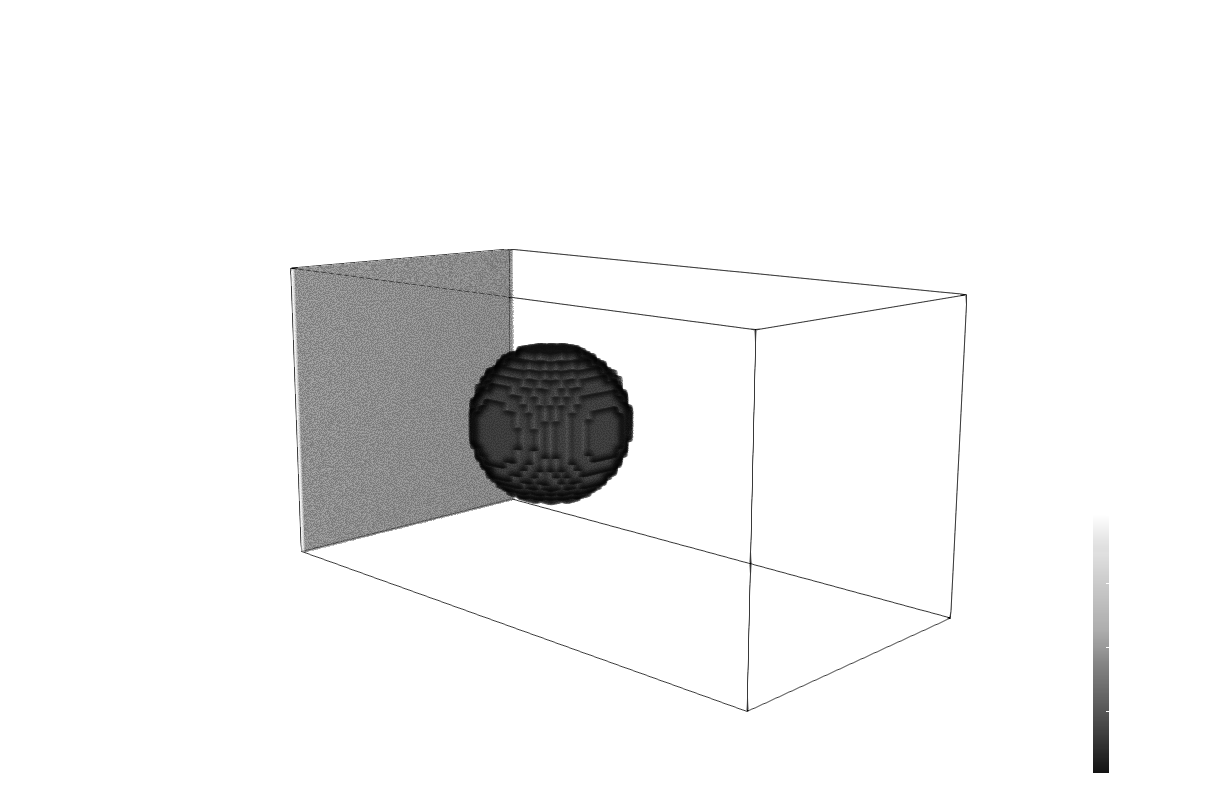
\includegraphics[width=0.7\linewidth]{figures/sphere_paraview.png}    
    \caption{Caption}
    \label{fig: Sphere simulation domain}
\end{figure}

The outlined procedure can be extended to simulate more complex geometries commonly found in practical applications, such as those encountered in gridded electrostatic ion thrusters. In those systems, positively charged ions are accelerated and precisely focused by a series of 2 or 3 grids, each containing typically thousands of coaxial apertures \cite{noauthor_gridded_nodate}. The ions are accelerated due to the potential difference between the first and the second grid, known as the screen and the accelerator grid, respectively \cite{foster_review_2024}. Simulating these ion thrusters accurately requires modeling variations in the thickness and size of the grid structure, as well as the electric potential applied to each grid. A simplistic version of such a grid aperture can be implemented using the following approach:
\begin{figure}[H]
    \centering
    \begin{lstlisting}
def add_plane_with_hole(self, z_0, thickness, phi_plane, hole_0,hole_r):

# Loop over all nodes
for i in range(self.ni):
    for j in range(self.nj):
        for k in range(self.nk):
            x, y, z = self.pos(i, j, k)  # coordinates of the current node
            
            # Calculate the distance from the hole-center in the XY plane
            xy_dist2 = (x - hole_0[0]) ** 2 + (y - hole_0[1]) ** 2
            
            # Check if the current node is within the plane thickness
            # and outside the circular hole area
            if z_0 <= z < (z_0 + thickness) and xy_dist2 > hole_radius2:
                self.objectid.data[i, j, k] = 1  # Set object flag
                self.phi.data[i, j, k] = phi_plane  # Set potential
    \end{lstlisting}
    \caption{Caption}
    \label{fig:enter-label}
\end{figure}

Such a system can be effectively visualized using ParaView, providing a detailed representation of the grid structure and particle dynamics. The following illustration demonstrates two grids with apertures of varying plane thickness and size. On the left side of the simulation domain is an inlet, from which charged particles could be injected at a specified drift velocity:
\begin{figure}[H]
    \centering
    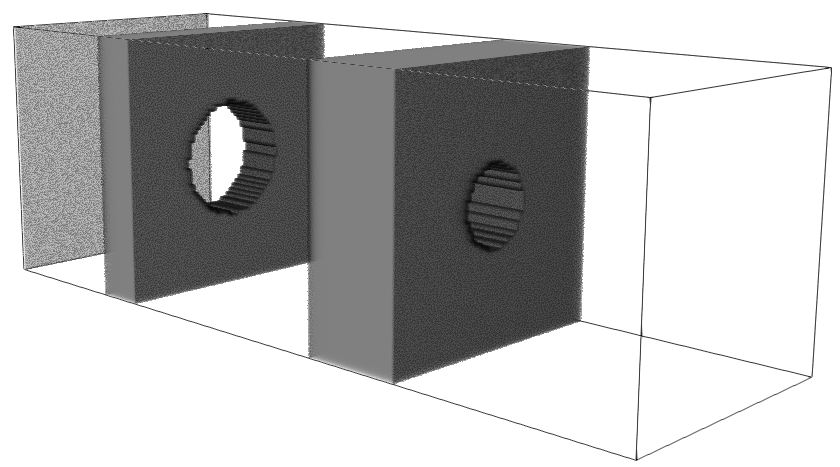
\includegraphics[width=0.7\linewidth]{figures/GIT_Paraview.png}
    \caption{Caption}
    \label{fig:enter-label}
\end{figure}
\section{Optimizing of the Relaxation Factor}
\label{Sec: Optimizing Relaxation Factor}

\usepackage{graphicx}   % For including graphics
\usepackage{subcaption} % For subfigures

\begin{figure}[H]
    \centering
    \begin{subfigure}[b]{0.55\linewidth}
        \centering
        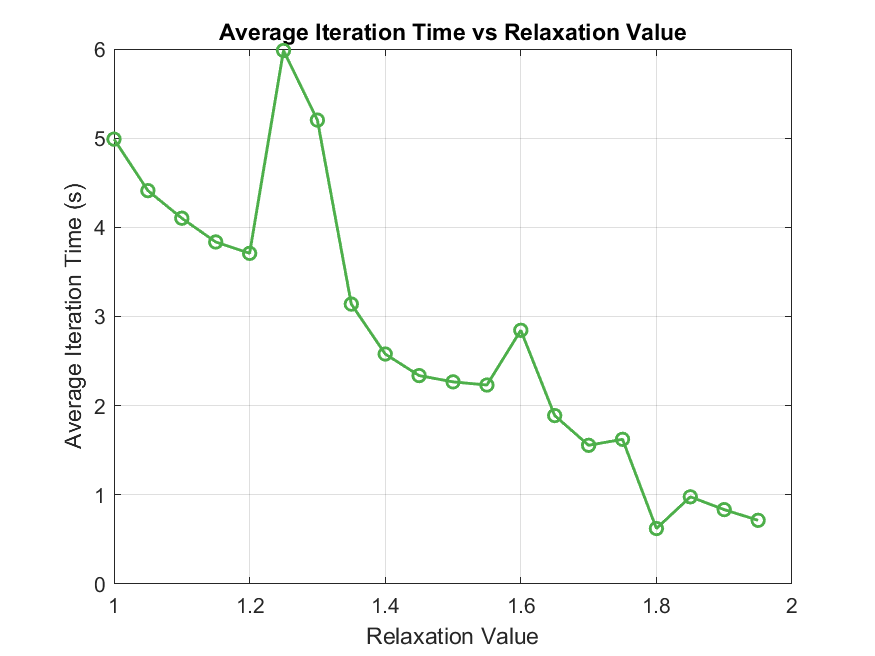
\includegraphics[width=\linewidth]{figures/overrelaxation/average_iteration_time_vs_relaxation_value.png}
        \caption{Average Iteration Time vs Relaxation Value}
        \label{fig:average_iteration_time}
    \end{subfigure}
    \hfill
    \begin{subfigure}[b]{0.55\linewidth}
        \centering
        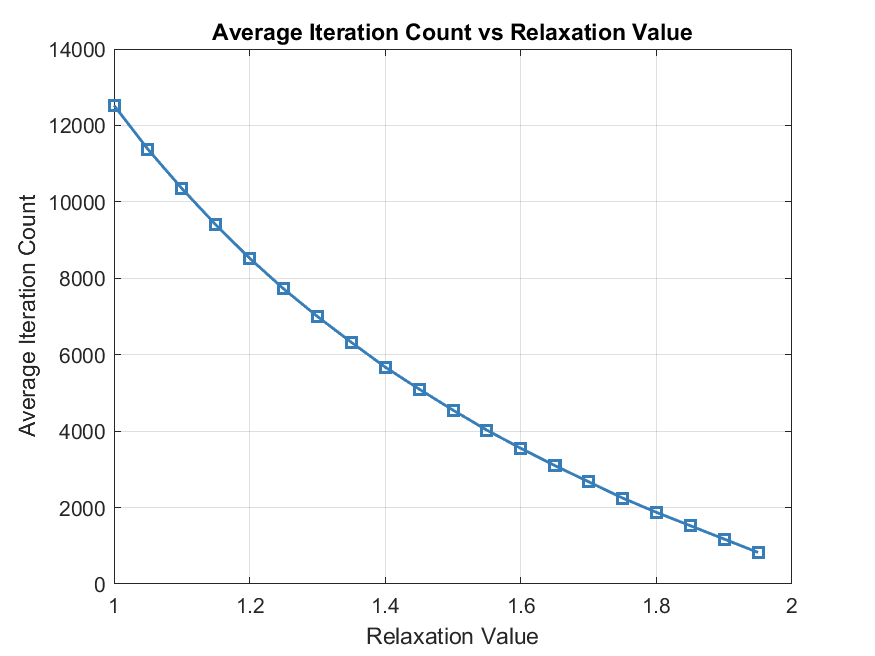
\includegraphics[width=\linewidth]{figures/overrelaxation/average_iteration_count_vs_relaxation_value.png}
        \caption{Average Iteration Count vs Relaxation Value}
        \label{fig:average_iteration_count}
    \end{subfigure}
    \caption{Comparison of Average Iteration Time and Count with Relaxation Values}
    \label{fig:comparison}
\end{figure}

\section{Simulation Outcomes}\label{Sec: Simulation Outcomes}

This section presents the simulation outcomes for two specific cases: the flow of charged particles around a sphere and the behavior of ions in a grid potential layout similar to those found in gridded electrostatic ion thrusters. These simulations are evaluated by examining energy conservation within the system, serving as a key indicator to verify the plausibility of the results. Furthermore, the steady state of the simulation is introduced, where key properties of the system, such as mass, momentum, energy, and charge, become time-invariant. This condition defines the point at which further iterations no longer provide significant changes to the results, indicating the simulation has reached equilibrium. Lastly, the limitations of the current implementation of the electrostatic particle-in-cell (\acs{ES PIC}) method are outlined and demonstrated through a specific challenge encountered during simulation.

\subsection{Flow Around a Sphere}\label{Sec: Flow Around Sphere}

In this section, a sphere with a fixed potential of $\Phi = -100V$ is introduced within the simulation domain, as illustrated in Fig. \ref{fig: Sphere simulation domain}. Oxygen ions (O+) with a single positive charge are injected from the inlet on the left plane, maintaining a particle density of \SI{1e10}{\per\meter^3} and a drift velocity of 7000 m/s. The sphere serves as a particle sink, absorbing ions upon interaction. As a result, a condensed stream forms behind the sphere, characterized by a region of increased ion density. This phenomenon arises due to the lensing effect, where the sphere deflects ion trajectories, concentrating them in the region downstream \cite{brieda_plasma_2019}.

\begin{figure}[H]
    \centering
    \begin{subfigure}[b]{0.49\linewidth}
        \centering
        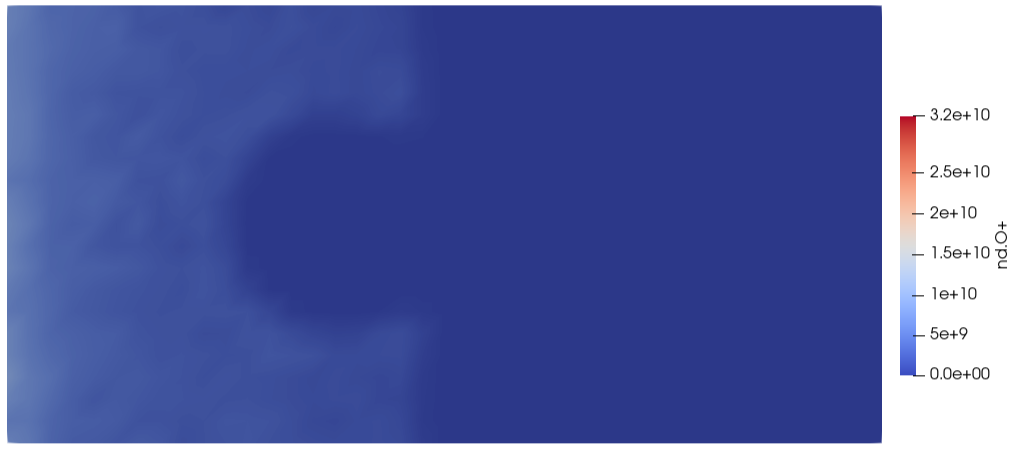
\includegraphics[width=\linewidth]{figures/Sphere/80_iterations.png}
        \caption{80 Iterations}
        \label{fig:average_iteration_time}
    \end{subfigure}
    \hfill
    \begin{subfigure}[b]{0.49\linewidth}
        \centering
        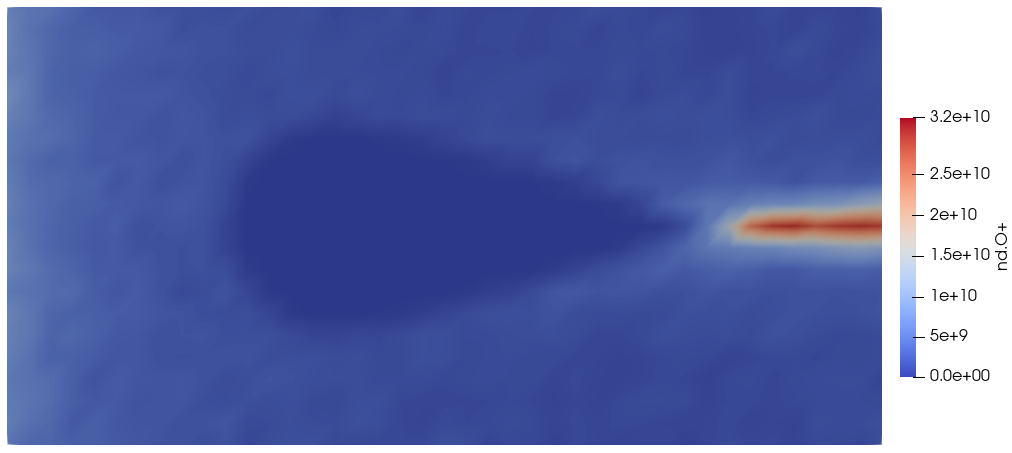
\includegraphics[width=\linewidth]{figures/Sphere/160_iterations.png}
        \caption{160 Iterations}
        \label{fig:average_iteration_count}
    \end{subfigure}
    \caption{Comparison of Average Iteration Time and Count with Relaxation Values}
    \label{fig:comparison}
\end{figure}


steady state 

only changes through noise introduced by the randomized injection of particles!

Therefore some fluctuations


\begin{figure}[H]
    \centering
    \begin{subfigure}[b]{0.49\linewidth}
        \centering
        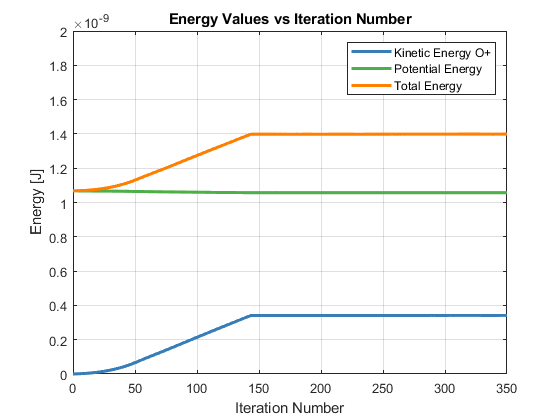
\includegraphics[width=\linewidth]{figures/Sphere/energy_values_plot.png}
        \caption{Energy}
        \label{fig:average_iteration_time}
    \end{subfigure}
    \hfill
    \begin{subfigure}[b]{0.49\linewidth}
        \centering
        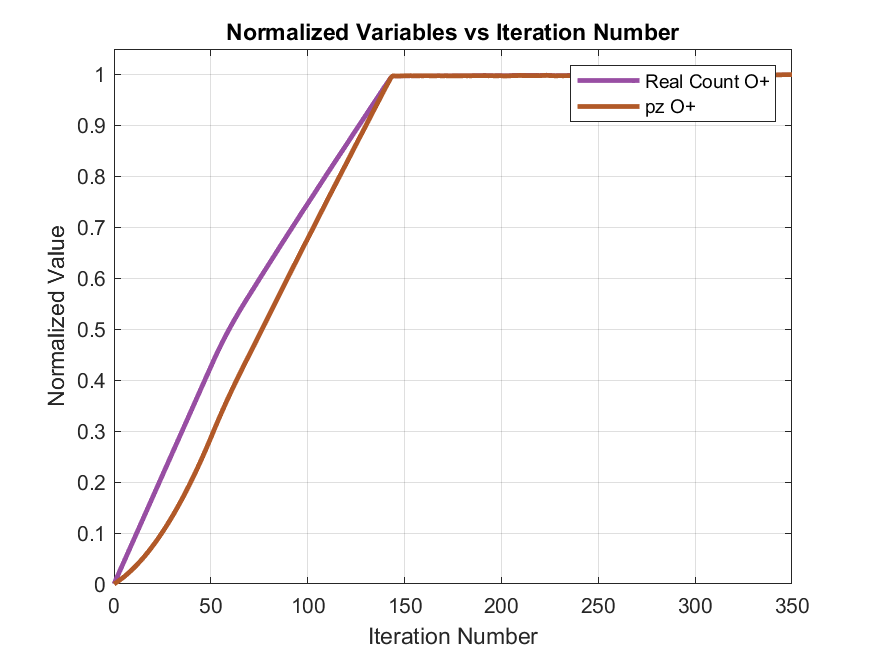
\includegraphics[width=\linewidth]{figures/Sphere/normalized_variables_plot.png}
        \caption{other variables}
        \label{fig:average_iteration_count}
    \end{subfigure}
    \caption{Comparison of Average Iteration Time and Count with Relaxation Values}
    \label{fig:comparison}
\end{figure}

Expected results the potential energy resulting from the grids remains constant in the system

however the kinetic energy and therefore the the total energy in the system increases until the steady state is achieved.

This happens after roughly 145 iterations at which point the total amount of particles in the system remains the same.

Those outcomes are consistent with the results presented for a similar simulation outlined in \cite{brieda_plasma_2019}.

\subsection{Basic Framework for Grid Potential Layout in RIT Thruster Design}
\section{Discussion}\label{Sec: Discussion}

\chapter{Future Work}
\chapter{Conclusion}
% Hier wird das Literaturverzeichnis eingebunden
%\printbibliography


\printbibliography[title={Bibliography}, heading=bibintoc]

\cleardoublepage

\appendix

%\chapter{Ergänzende Informationen 1}
%\blindtext


\end{document} 